\documentclass[11pt, openany]{book}
\setcounter{tocdepth}{3}
\setcounter{secnumdepth}{3}
\usepackage[italian]{babel}
\usepackage{subfigure}
\usepackage[a4paper,top=3cm,bottom=3cm,left=2cm,right=2cm,marginparwidth=2cm]{geometry}
\usepackage{tocbibind}
\usepackage{listings}
\usepackage{xcolor}
\usepackage{midpage}
\renewcommand{\lstlistingname}{Algoritmi}
\renewcommand{\lstlistlistingname}{Lista degli \lstlistingname}
\usepackage{listings}
\usepackage{xcolor}
\definecolor{bluekeywords}{rgb}{0.13,0.13,1}
\definecolor{greencomments}{rgb}{0,0.5,0}
\definecolor{turqusnumbers}{rgb}{0.17,0.57,0.69}
\definecolor{redstrings}{rgb}{0.5,0,0}
\lstset{language=[Sharp]C,
captionpos=b,
%numbers=left, %Nummerierung
%numberstyle=\tiny, % kleine Zeilennummern
frame=lines, % Oberhalb und unterhalb des Listings ist eine Linie
showspaces=false,
showtabs=false,
breaklines=true,
showstringspaces=false,
breakatwhitespace=true,
escapeinside={(*@}{@*)},
commentstyle=\color{greencomments},
morekeywords={partial, var, value, get, set},
keywordstyle=\color{bluekeywords},
stringstyle=\color{redstrings},
basicstyle=\ttfamily\small,
}
\lstloadlanguages{csh}
\usepackage{titlesec}
\usepackage{imakeidx}
\usepackage{amsmath}
\usepackage{graphicx}
\usepackage{blindtext}
\usepackage{lastpage}
\pagestyle{plain}
\usepackage[utf8]{inputenc}
\usepackage{float}
\usepackage{sidecap, caption}
\usepackage{setspace}
\usepackage{url}
\usepackage{hyperref}
\usepackage[xindy,toc]{glossaries}
\loadglsentries{glossario}
\usepackage[sorting=none, block = ragged]{biblatex}
\addbibresource{Bibliografia.bib}
\graphicspath{ {./images/} }
\makeglossaries
\linespread{1.1}
\begin{document}
\begin{titlepage}
\begin{SCfigure}[14.5][h]
            \caption*{
                Università degli studi di Milano Bicocca \\
                \textbf{Scuola di Scienze} \\
                \textbf{Dipartimento di Informatica, Sistemistica e Comunicazione} \\
                \textbf{Corso di Laurea in Informatica} \\
                }
            
\includegraphics[]{Immagini/logo_bicocca.png}
\end{SCfigure}
\begin{center}
        \vspace{2cm}
        \textbf{\Huge
        Integrazione di funzionalità interattive\\in un ambiente di realtà virtuale multi-utente}
        \vspace{4cm}
        \begin{FlushLeft}
        \Large
            \textbf{Relatore: } \textit{Prof. Giuseppe Vizzari}
            \\
            \textbf{Co-relatrice: } \textit{Prof.ssa Daniela Briola}
        \end{FlushLeft}

        \vspace{2cm}
        \begin{FlushRight}
        \Large
            \textbf{Relazione della prova finale di}
            \\
            \textit{Ghezzi Davide \\ Matricola 846114}
        \end{FlushRight}

        \large \vspace*{\fill} Anno Accademico 2021 - 2022
    \end{center}
\newpage
\end{titlepage}
\newpage
\begin{midpage}
\begin{center}
\begin{FlushRight}
 \textit{Alla mia famiglia che mi ha sempre supportato ed incoraggiato \\nelle mie
scelte e nello studio.
\\Ai miei amici che ogni giorno hanno condiviso con me momenti di gioia, \\sostenendomi nei periodi di sconforto e non voltandomi mai le spalle.
\\A tutti i professori e ai ricercatori che hanno contribuito alla mia \\formazione culturale e professionale}.   
\end{FlushRight}
\end{center}
\end{midpage}
\tableofcontents
\listoffigures
\printglossaries
\chapter{Introduzione}
Nel corso degli ultimi vent'anni abbiamo assistito ad uno sviluppo esponenziale della tecnologia che ha portato una fetta sempre più grande di pubblico a disporre di hardware con potenza di calcolo elevata ad un costo relativamente contenuto.
\\Basti pensare, ad esempio, alle TV o telefoni cellulari disponibili agli inizi degli anni 2000 che non possono assolutamente competere con i rispettivi prodotti disponibili attualmente sul mercato.
\\Di conseguenza, le persone al giorno d'oggi hanno anche a disposizione software molto più complessi e avanzati rispetto al recente passato, grazie ai quali possono affacciarsi sempre più frequentemente a nuove tecnologie.
\\Una delle tecnologie che ha prepotentemente preso piede negli ultimi anni è la \textbf{Realtà Virtuale}.
\\La Realtà Virtuale (\textit{Virtual Reality}) è una realtà simulata, un mondo digitale dove si viene immersi indossando un apposito visore, che avvolge totalmente l'utente, andando a mascherare del tutto la percezione, quantomeno visiva, del mondo fisico intorno a lui.
\\È una tecnologia impiegata soprattutto in ambito videoludico, ma è molto utile anche in ambito didattico, perché è possibile vivere delle esperienze educative grazie alla riproduzione fedele di luoghi storici come monumenti, luoghi di culto, siti archeologici oppure luoghi naturali come fondi oceanici, sentieri montuosi, siti geologici.
\\Al giorno d'oggi, esistono molteplici applicazioni in realtà virtuale in grado di far vivere all'utente le esperienze viste in precedenza e in cui può anche muoversi per esplorare l'ambiente o interagire con esso.\footnote{\url{https://www.lifewire.com/virtual-reality-tourism-4129394} in questo sito web sono illustrate alcune applicazioni di questo tipo}
\\Queste applicazioni, seppur molto utili per l'apprendimento didattico individuale, presentano un grosso problema: non supportano la presenza di più utenti, ma, come ben sappiamo, in un'aula scolastica solitamente sono presenti un docente e circa venti studenti. 
\\Di conseguenza, le caratteristiche principali che un'applicazione multi-utente deve avere sono:
\begin{itemize}
    \item Percezione contemporanea degli utenti e delle loro azioni;
    \item Interazione con l'ambiente, con modifiche visibili a tutti;
    \item Possibilità di interagire con gli altri utenti attraverso una chat di testo o vocale (data la difficoltà d’uso di meccanismi di input-output tradizionali mentre si utilizza un visore).
\end{itemize}
Lo scopo del progetto è innanzitutto quello di analizzare le soluzioni tecnologiche e programmative per risolvere il problema della mono-utenza, con il fine di rendere effettivamente utili questo tipo di applicazioni per l'apprendimento scolastico, infine quello di ricreare un ambiente che mostri il funzionamento delle suddette soluzioni tramite la realizzazione di un prototipo.
\section{Requisiti}
Con le premesse esposte in precedenza, si è voluto realizzare un prototipo di un ambiente di realtà virtuale multi-utente che potesse ospitare circa una ventina utenti, di cui un docente.
\\Ogni utente ha la percezione visiva e uditiva di ciò che lo circonda, compresi gli altri utenti, per ricreare al meglio la sensazione di presenza e partecipazione all'interno dell'aula virtuale.
\\Inoltre, al docente è stata data la possibilità di poter disattivare o attivare il microfono di uno o più utenti a suo piacimento ed è stata introdotta anche la possibilità per ogni altro utente di richiedere la parola, proprio come uno studente quando in un aula scolastica \textit{`alza la mano`}.
\\La grossa differenza rispetto ad un'aula scolastica risiede nell'ambiente in cui tutti gli utenti sono immersi. 
\\In questo prototipo gli utenti verranno immersi in un ambiente naturale con un castello medioevale esplorabile, questo modello è stato scelto semplicemente per dare un’idea delle possibilità grafiche e farsi un’idea dei costi computazionali, senza aver valutato approfonditamente un contesto disciplinare formativo.
\\L'ambiente in questione potrebbe essere utile, per esempio, per una lezione di storia, arte o architettura.
\\Questa particolarità ha portato alla luce un'ulteriore requisito, ovvero la possibilità per il docente di interagire con l'ambiente circostante.
\\Per il docente, durante la simulazione, può essere molto utile segnalare o indicare particolari luoghi all'interno dell'ambiente, a tale scopo è stata pensata la possibilità di poter piazzare e rimuovere delle bandierine dai suddetti luoghi.
\\Per concludere, visto la mancata possibilità di disporre di un ambiente virtuale che riproducesse fedelmente un ambiente reale, l'ambiente sviluppato è a scopo illustrativo e ancora allo stato primordiale.
\section{Realizzazione}
Il prototipo è stato realizzato in collaborazione con due colleghi del Dipartimento di Informatica Sistemistica e Comunicazione dell'Università degli studi di Milano-Bicocca, Emanuele Sapio e Lorenzo Iacopetta.
\\Le prime fasi di sviluppo sono state caratterizzate da ricerche approfondite che hanno poi portato ad una suddivisione dei compiti per accelerare la fase di sviluppo del software.
\\In particolare, i miei colleghi hanno approfondito la parte di \textit{\gls{networking}}, cioè di connessione tra i dispositivi degli utenti, e della chat vocale, attraverso l'uso delle librerie: \textbf{Photon PUN} e \textbf{Photon Voice}.
\\La parte sviluppata da me, invece, riguarda: l'interazione con l'ambiente da parte del docente, l'implementazione di una chat testuale e l'implementazione di una schermata per l'attivazione e la disattivazione del microfono degli utenti.
\section{Organizzazione dei Capitoli}
In questa relazione sono presenti altri 5 Capitoli oltre a questo capitolo introduttivo.
\\Nel \textbf{Cap.2} sarà presentata la fase di analisi e progettazione del prototipo.
\\Nel \textbf{Cap.3} si analizzeranno le Tecnologie abilitanti, ovvero gli strumenti che sono stati utilizzati per la progettazione e sviluppo del prototipo.
\\Nel \textbf{Cap.4} verrà illustrata la parte del prototipo sviluppata dal sottoscritto.
\\Nel \textbf{Cap.5} verrà mostrato il funzionamento delle parti fondamentali del prototipo attraverso alcune dimostrazioni d'uso.
\\Nel \textbf{Cap.6} saranno presentati alcuni possibili sviluppi futuri del prototipo e delle sue funzionalità. 

\chapter{Analisi e Progettazione}
Come anticipato nel capitolo introduttivo, il progetto prevede la creazione di un'aula virtuale in cui il docente e gli studenti possono comunicare tra loro e interagire con l'ambiente circostante.
\\In questo capitolo verrà illustrata prima la fase di analisi, attraverso la specifica dei requisiti e dei casi d'uso, successivamente la fase di progettazione, con i diagrammi di \textbf{\textit{workflow}} (flussi di lavoro).
\section{Specifica dei Requisiti}
L'analisi dei requisiti funzionali, ha fatto emergere alcune delle proprietà che il sistema deve necessariamente avere per soddisfare la richiesta.
\\La prima proprietà riguarda gli attori del sistema, secondo la specifica, infatti, è necessario distinguere due attori:
\begin{itemize}
    \item Docente
    \item Studente
\end{itemize} 
Questa distinzione implica la necessità di introdurre un sistema di autenticazione
in modo tale da poter identificare l'utente e il suo ruolo all'interno
dell'applicazione.\\
Una seconda proprietà emersa riguarda il tipo di interazioni che gli attori
possono avere tra loro, perciò è stato introdotto un mezzo di comunicazione fra utenti connessi.
\\Infine, è stato necessario introdurre un sistema che permettesse agli utenti
di interagire con l'ambiente circostante, in particolare il docente deve avere la
possibilità di indicare un punto di interesse all'interno della scena virtuale.\\
Questa breve descrizione delle funzionalità richieste ci permette di identificare
più in dettaglio i requisiti funzionali:
\begin{itemize}
    \item Il sistema deve permettere l'identificazione dell'utente, in modo da poterne
     stabilire il ruolo; 
     \item Il sistema deve consentire agli attori di accedere ad uno spazio comune e
di potersi vedere reciprocamente;
     \item All'interno dello spazio comune il sistema deve fornire uno strumento di
comunicazione agli utenti;
     \item All'interno dello spazio comune il sistema deve prevedere la possibilità, da
parte del docente, di indicare un punto di interesse.
\end{itemize} 
Un forte vincolo imposto all'applicazione è rappresentato dall'assenza di un'iscrizione o registrazione.\\ Per semplicità, si è deciso di trascurare questa funzionalità aggiuntiva che necessiterebbe di un \gls{database}, per memorizzare i dati di accesso degli utenti, e di una funzionalità per l'accesso ai dati.
\\Le credenziali di autenticazione sono specificate in un file json.
\section{Analisi dei casi d'uso}
La specifica dei requisiti indica chiaramente la presenza di due attori che condividono alcune funzionalità comuni, pertanto è stata creata una generalizzazione, chiamata Utente, di questi due attori.
\begin{figure}[H]
    \centering
    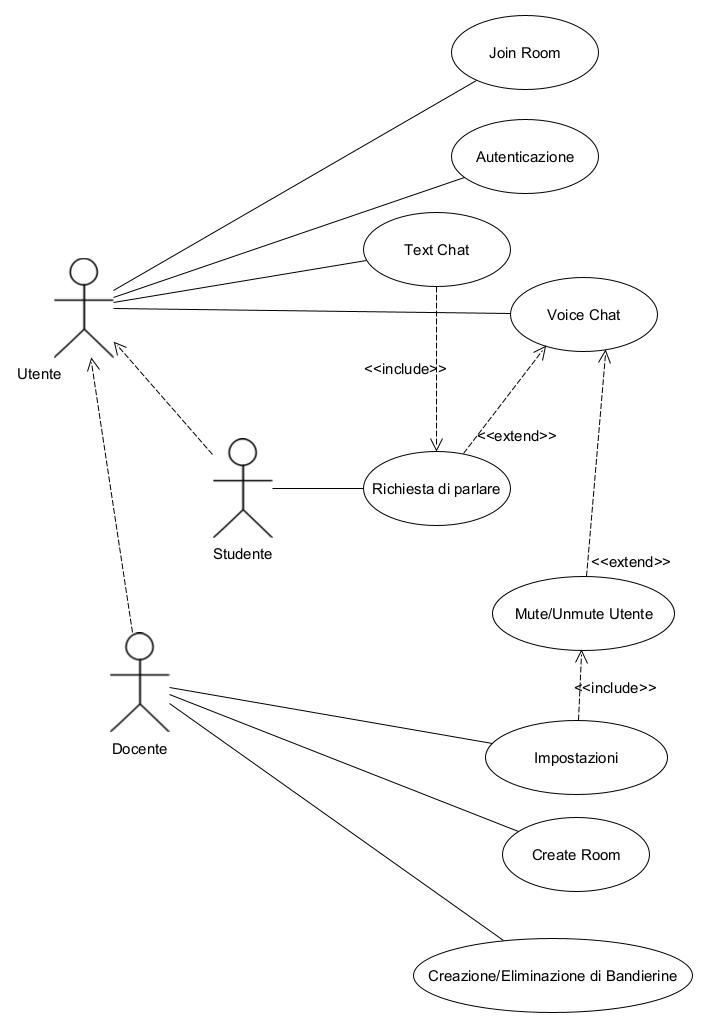
\includegraphics[width = 14cm, height = 17cm]{Immagini/AppUseCase (complete).jpg}
    \caption{Diagramma completo dei casi d'uso }
    \label{fig:my_label}
\end{figure} 
\hspace*{-0.6cm}Dalle specifiche dei requisiti sono stati identificati 9 casi d'uso, ovvero la descrizione di un insieme di interazioni, tra un utente ed un sistema, che consentono all'utente di raggiungere un obiettivo o di svolgere un compito:
\begin{itemize}
\item Autenticazione;
\item Create Room;
\item Join Room;
\item Chat Vocale;
\item Chat di testo;
\item Richiesta di parlare;
\item Impostazioni;
\item Mute/Unmute Utente;
\item Creazione/Eliminazione di bandierine.
\end{itemize}
\subsection{Autenticazione}
Dalle specifiche risulta evidente  la  necessità  di  distinguere  gli utenti  in  due  attori, perciò è stato introdotto un meccanismo di autenticazione necessario per la verifica dell'identità dell'utente.
\\Il caso d'uso \textit{Autenticazione} inizia in seguito all'avvio dell'applicazione, dopodiché l'attore inserisce le proprie credenziali, ovvero \textit{username} e \textit{password} e clicca sul bottone \textit{login}.
\\Se le credenziali sono errate, il sistema mostrerà un messaggio di errore, se invece l'autenticazione ha successo, l'attore verrà indirizzato verso una nuova scena che differisce a seconda del ruolo in cui si è identificato.
\begin{figure}[H]
    \centering
    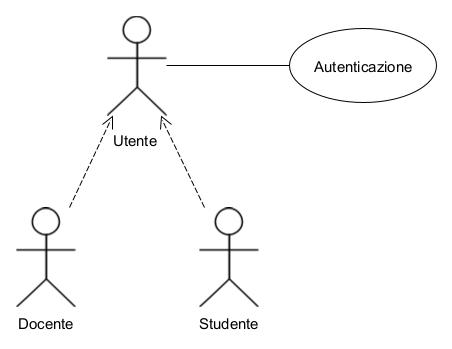
\includegraphics[scale=0.5]{Immagini/LoginUseCase.jpg}
    \caption{Diagramma del caso d'uso Autenticazione}
    \label{fig:my_label}
\end{figure}
\subsection{Create Room}
Il caso d'uso \textit{Create Room} ha come precondizione aver effettuato l'autenticazione con successo con il ruolo di docente.
\\Il sistema mostra all'attore una schermata con la lista delle aule già create, se presenti, e offre la possibilità di creare una nuova aula, assegnandole un nome. \\In seguito alla creazione della stanza, il docente viene automaticamente indirizzato alla scena relativa all'aula appena creata.\\Pertanto, sia che il docente crei una nuova stanza oppure scelga di entrare in un'aula già presente, il sistema caricherà la scena corretta per l'attore.
\subsection{Join Room}
\begin{figure}[H]
    \centering
    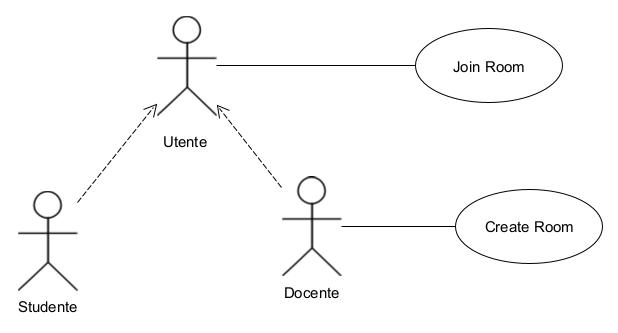
\includegraphics[scale=0.6]{Immagini/CreateJoinRoomUseCase.jpg}
    \caption{Diagramma dei casi d'uso Join Room e Create Room}
    \label{fig:my_label}
\end{figure}
Il caso d'uso \textit{Join Room} ha come precondizione aver effettuato l'autenticazione con successo con uno dei ruoli resi a disposizione dal sistema.
\\Il sistema presenta una schermata in cui viene mostrato l'elenco delle aule già disponibili. \\L'utente può scegliere tra le aule presenti ed entrare in una di queste, cliccando direttamente sul nome dell'aula.
\\Nel caso di un docente, l'ingresso in una stanza verrà effettuato non solo attraverso la scelta tra quelle disponibili, ma anche dopo aver effettuato la creazione di una nuova stanza.
\subsection{Chat Vocale}
Il caso d'uso \textit{Chat Vocale} ha come precondizione l'accesso ad uno spazio condiviso da due o più utenti. \\In questa fase non sono richieste particolari azioni da parte degli attori, ma risulta importante evidenziare come essi ottengano valore da questo caso d'uso, infatti è da questo che gli utenti ottengono la possibilità di comunicare tra loro tramite i microfoni e le cuffie.
\\Non appena gli attori accedono alla stessa aula, il sistema permette loro di comunicare e di vivere un'esperienza audio realistica attraverso la tecnologia \textbf{audio 3D}, che consente all'ascoltatore di percepire il suono da ogni direzione.
\subsection{Chat di testo}
Il caso d'uso \textit{Chat di testo} ha come precondizione l'accesso ad uno spazio condiviso da due o più utenti.
\\Il sistema garantisce una comunicazione network attraverso un'interfaccia utente nella quale è possibile scrivere dei messaggi e inviarli agli altri utenti.
\subsection{Richiesta di parlare} \label{Request}
\begin{figure}[H]
    \centering
    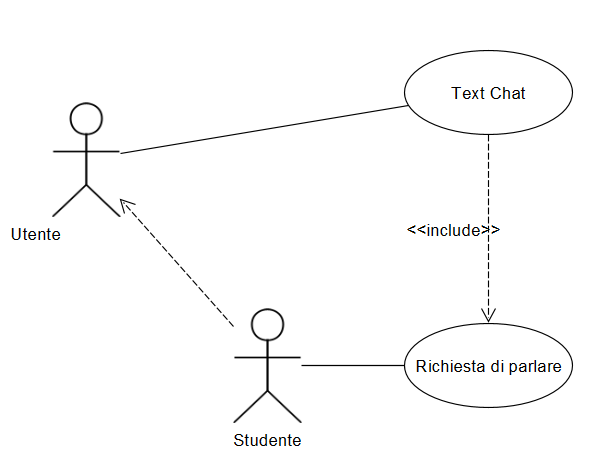
\includegraphics[scale=0.6]{Immagini/text.jpg}
    \caption{Diagramma del caso d'uso Text Chat che include Richiesta di Parlare}
    \label{fig:my_label}
\end{figure}
Il caso d'uso \textit{Richiesta di Parlare} ha come precondizione l'accesso ad uno spazio condiviso da due o più utenti e che l'attore di questo caso d'uso abbia il ruolo di studente.
\\Come detto in precedenza, all'interno dell'aula, il docente avrà l'autorità di concedere la parola ad uno studente, a tutti, oppure togliere questo diritto a sua discrezione. \\Questo potrebbe portare ad una comunicazione unilaterale in cui gli studenti sono attori passivi della comunicazione. \\Per ovviare a questo possibile inconveniente, gli studenti hanno la possibilità di richiedere la parola. \\Per fare ciò, nella schermata della chat di testo presentata dal sistema, sarà presente un bottone che invierà sulla chat una notifica, della forma: \textit{`Nome studente} richiede di parlare`, a tutti gli utenti. \\A questo punto il docente può decidere se concedere la parola allo studente che l'ha richiesta.
\subsection{Impostazioni}
Il caso d'uso \textit{Impostazioni} ha come precondizione l'accesso ad uno spazio condiviso da due o più utenti e che l'attore di questo caso d'uso abbia il ruolo di docente.
\\Il sistema mostrerà al docente una schermata, che possiede l'elenco dei nomi dei giocatori connessi alla stanza, nella quale sono abilitate le funzioni del caso d'uso \textit{Mute/Unmute Utente}.
\subsection{Mute/Unmute Utente}
Il caso d'uso \textit{Mute/Unmute Utente} ha come precondizione l'accesso ad un'aula da parte di più utenti e che l'attore di questo caso d'uso abbia il ruolo di docente. \\All'interno dell'aula, il docente avrà l'autorità di concedere la parola ad uno studente, a tutti, oppure togliere questo diritto a sua discrezione. \\Il docente avrà la possibilità di vedere l'elenco degli studenti presenti nell'aula e, accanto ai loro nomi, sarà presente un bottone che permetterà di dare e togliere la parola al relativo studente.
\begin{figure}[H]
    \centering
    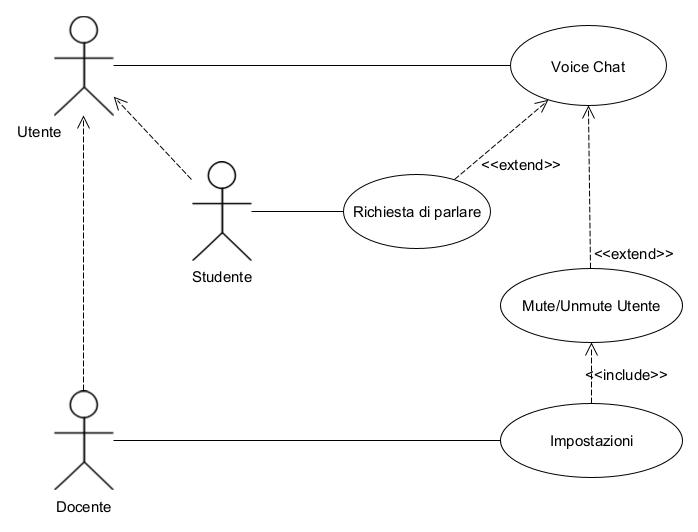
\includegraphics[scale=0.6]{Immagini/VoiceChatUseCase.jpg}
    \caption{Diagramma dei casi d'uso Voice Chat, Mute/Unmute Utente, Impostazioni}
    \label{fig:my_label}
\end{figure}
\subsection{Creazione/Eliminazione di bandierine}
Il caso d'uso \textit{Creazione/Eliminazione di bandierine} ha come precondizione l'accesso ad un'aula da parte di più utenti e che l'attore di questo caso d'uso abbia il ruolo di docente.
\\Il caso d'uso modella l'interazione con l'ambiente circostante, ovvero con gli elementi presenti nell'aula. \\Questa interazione si è tradotta nella possibilità di inserire, in alcuni punti prestabiliti, una bandierina. \\L'attore abilitato a questo caso d'uso deve indicare in direzione dell'area prestabilita e, cliccando all'interno di quell'area, può generare la bandierina. \\Ad un successivo click, all'interno dell'area, la bandierina viene rimossa.
\begin{figure}[H]
    \centering
    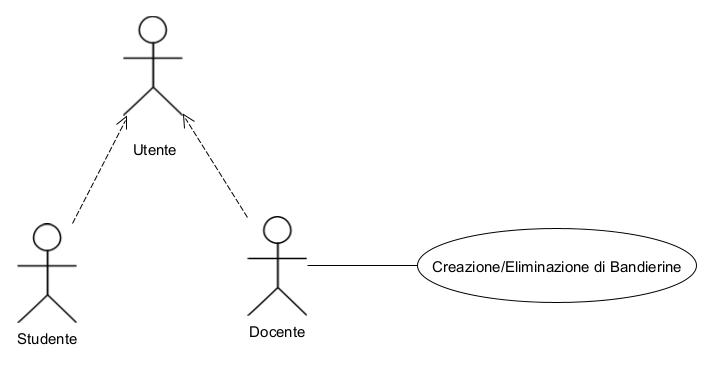
\includegraphics[scale=0.6]{Immagini/EnvironmentInteractionUseCase.jpg}
    \caption{Diagramma del caso d'uso Creazione/Eliminazione Bandierina}
    \label{fig:my_label}
\end{figure}
\section{Diagrammi Workflow}
La definizione dei casi d'uso porta a scomporre il progetto nelle sue parti costituenti. \\Ognuna di queste risponde ad una specifica necessità emersa dall'analisi dei requisiti. \\Molti casi d'uso si sono tradotti quasi direttamente in un diagramma \textit{workflow}, che mostra il flusso delle diverse attività in un caso d'uso. \\In particolare sono stati definiti 3 diagrammi \textit{workflow} che corrispondono a 3 casi d'uso descritti in precedenza:
\begin{itemize}
   \item Autenticazione Workflow;
   \item Create Room Workflow;
   \item Join Room Workflow.
\end{itemize}
L'analisi di questi 3 casi d'uso, più il caso d'uso \textit{Voice Chat}, verrà poi svolta più dettagliatamente dai colleghi Emanuele Sapio e Lorenzo Iacopetta nelle loro Relazioni, visto che riguarda la parte di cui si sono occupati nel progetto.
\\I rimanenti casi d'uso verranno analizzati dettagliatamente in un capitolo a parte, il \textbf{Cap.4}, per evidenziare meglio la parte del progetto svolta dal sottoscritto.
\subsection{Autenticazione}
\begin{figure}[H]
    \centering
    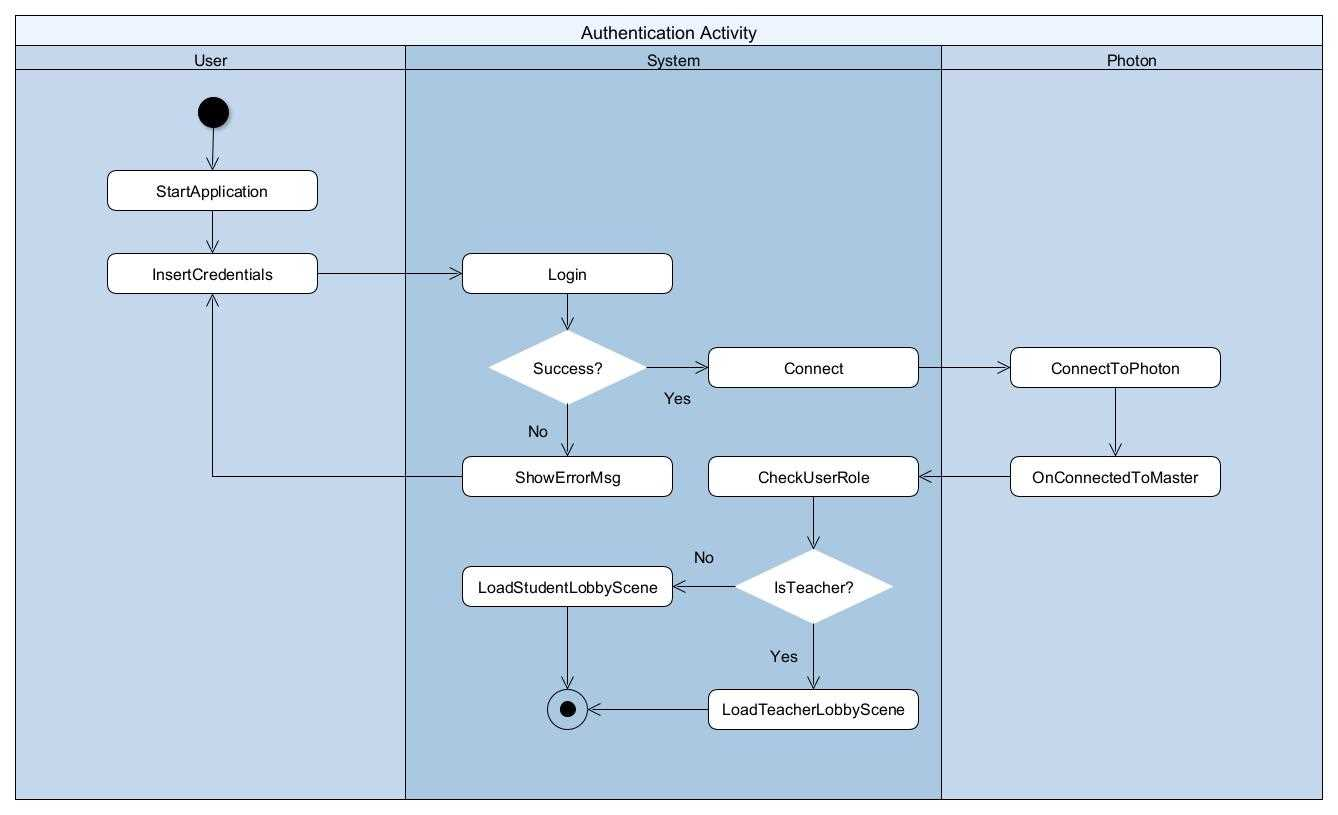
\includegraphics[width = 17cm, height = 14cm]{Immagini/AuthenticationActivityDiagram1.jpg}
    \caption{Diagramma Workflow di Autenticazione}
    \label{fig:my_label}
\end{figure}
L'autenticazione degli utenti ricopre un ruolo importante all'interno dell'applicazione, perché, in base al ruolo dell'attore, il sistema caricherà scene diverse e si avranno diritti e funzioni diverse.
\\Quando l'applicazione viene avviata, il sistema mostrerà all'utente una schermata in cui è possibile inserire le proprie credenziali ed effettuare l'accesso. 
\\In seguito al click dell'attore sul pulsante \textit{Login}, il sistema deve verificare che le credenziali siano corrette. 
\\Se l'utente non esiste nella base dati, il sistema deve restituire un messaggio di errore all'utente che può ripetere l'operazione, altrimenti il sistema si connette ad un server esterno (\textit{server Photon}).
\\Il server Photon possiede un identificativo, nascosto all'utente, che deve essere necessariamente impostato correttamente dal programmatore per poter permettere la comunicazione tra applicazioni diverse (e quindi utenti diversi), perciò le applicazioni con lo stesso identificativo si connetteranno allo stesso server di Photon.
\\In seguito alla connessione al server, il sistema verifica il ruolo dell'utente che si è appena collegato. 
\\Se si tratta di un docente, l'applicazione caricherà la scena dedicata ai docenti che permetterà, oltre ad accedere ad aule già presenti, la creazione di una nuova aula. 
\\Altrimenti, se l'attore è uno studente, il sistema caricherà la scena dedicata agli studenti, in cui è possibile scegliere ed entrare in un'aula.
\\Il flusso termina quando il sistema carica la scena appropriata per l'utente che si è collegato.
\subsection{Create Room}
\begin{figure}[H]
    \centering
    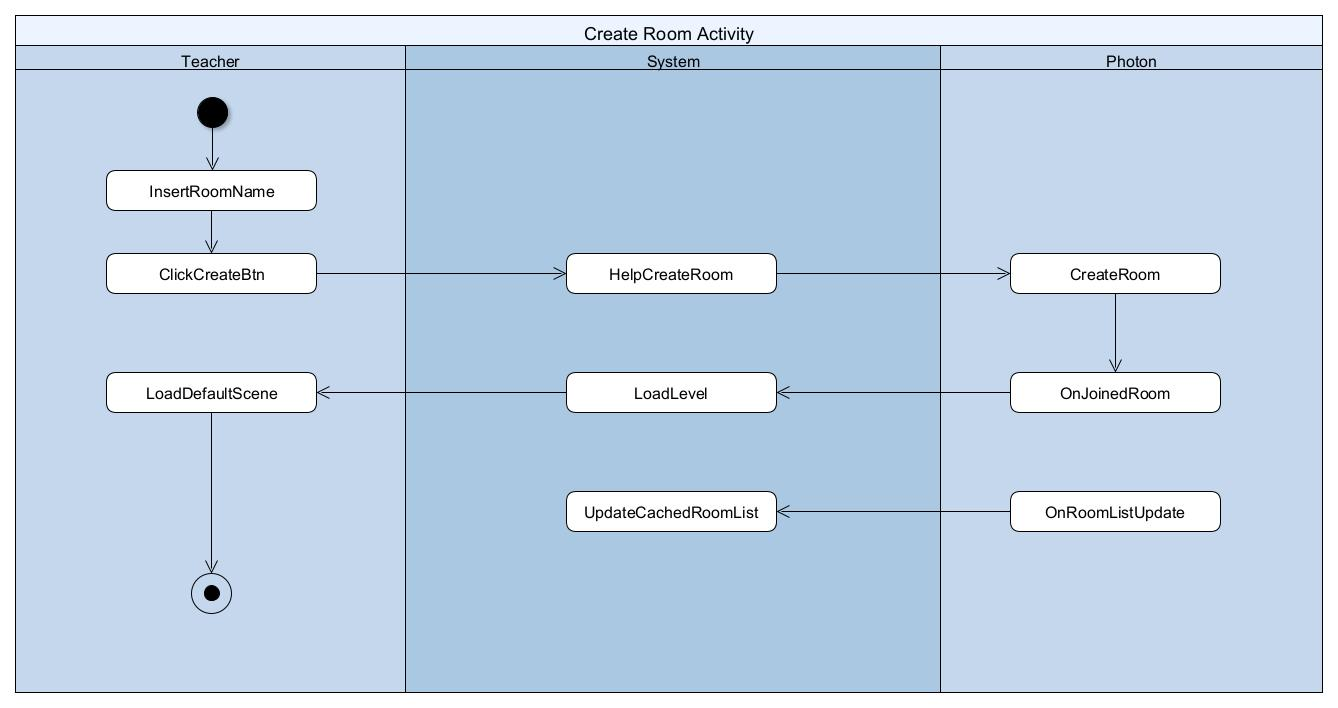
\includegraphics[width = 17cm, height = 13cm]{Immagini/CreateRoomActivityDiagram.jpg}
    \caption{Diagramma Workflow di Create Room}
    \label{fig:my_label}
\end{figure} 
In questo diagramma sono mostrate le attività che vengono svolte durante la creazione della stanza da parte del docente.
\\Il docente, innanzitutto, deve inserire un nome che verrà assegnato all'aula e cliccare sul bottone \textit{Create Room}.
\\Il sistema, a questo punto, invierà la richiesta di creazione di una stanza al server Photon che creerà un'istanza sul proprio server etichettata con il nome che il docente ha assegnato all'aula.
\\Dopodiché, il server Photon aziona una funzione di ingresso, per il docente, alla stanza appena creata, infine il sistema, sull'applicazione del docente, caricherà la scena in cui poi gli utenti andranno ad interagire.
\\La stanza creata dal docente sarà poi visibile a tutti gli altri utenti che accederanno alla scena adibita all'ingresso delle stanze virtuali, grazie all'operazione \textit{OnRoomListUpdate} del server Photon.
\subsection{Join Room}
\begin{figure}[H]
    \centering
    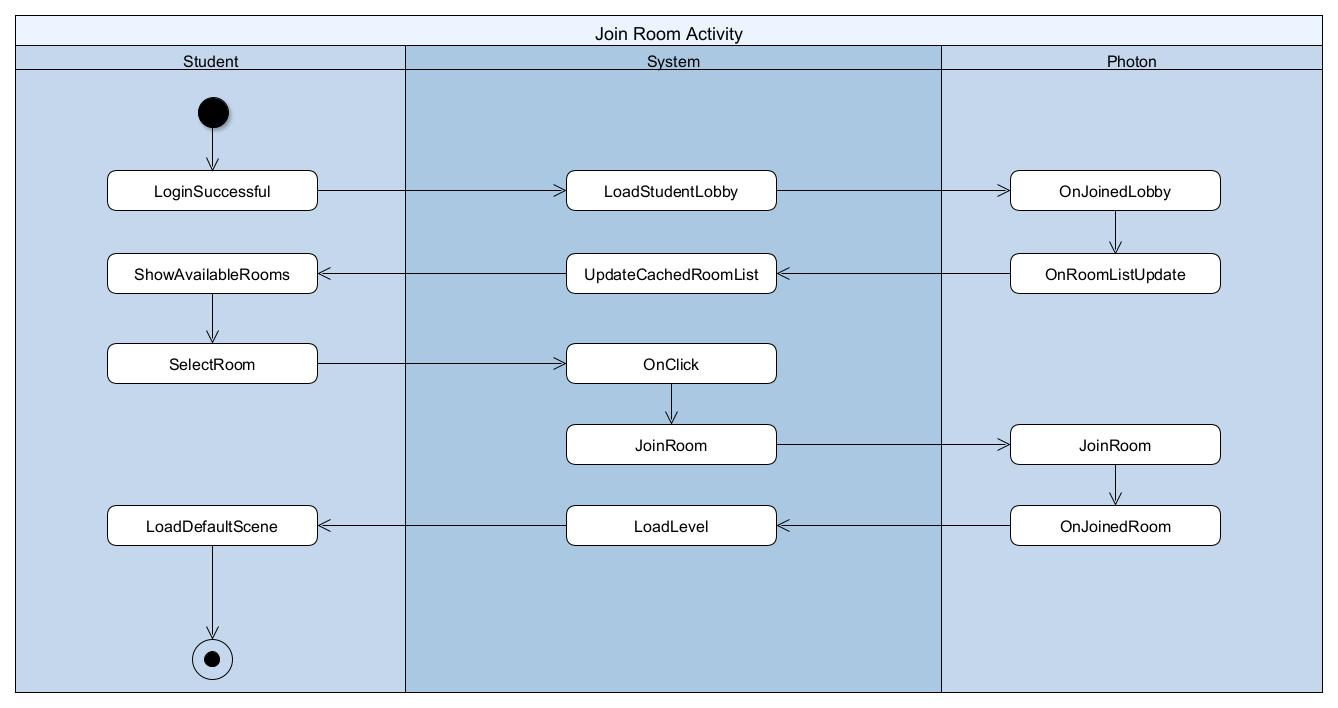
\includegraphics[width = 17cm, height = 13cm]{Immagini/JoinRoomActivityDiagram.jpg}
    \caption{Diagramma Workflow di Join Room}
    \label{fig:my_label}
\end{figure}
In questo diagramma sono illustrate le attività svolte durante l'operazione di collegamento ad una stanza creata. 
\\Come già accennato in precedenza, gli studenti visualizzeranno una scena in cui compare solo l'elenco delle aule disponibili, mentre gli insegnanti avranno anche la possibilità di creare una nuova aula. 
\\Come analizzato nel diagramma \textit{workflow} di Create Room, si tratta di una distinzione importante delle attività dell'applicazione rispetto a quelle del server Photon. 
\\L'accesso al server Photon, infatti, è del tutto trasparente all'utente perché è gestito dal server esterno.
\\Il compito del sistema, in questo caso, sarà quello di caricare e mostrare all'utente la lista delle stanze disponibili a cui si può collegare.
\\Una volta caricate le aule disponibili, l'utente può sceglierne una, e al click, l'applicazione invierà la richiesta di ingresso all'aula al server Photon. 
\\Sarà poi il sistema, in seguito all'attività del server, a caricare la scena relativa all'aula selezionata.
\\Quindi, ogni applicazione possiede una o più scene da caricare, quello che permette la comunicazione tra utenti è la connessione allo stesso server Photon.
\\Gli utenti potranno vedersi e interagire tra loro nella scena finale grazie alla presenza di un \textit{Avatar}: ogni utente possiede un \textit{Avatar} che è stato progettato con delle componenti \textit{sofware} in grado di renderlo percepibile a tutti gli altri utenti collegati alla stessa stanza virtuale.
\chapter{Tecnologie Abilitanti}
In questo capitolo verranno descritti gli strumenti e le tecnologie che sono stati utilizzati per la realizzazione dei requisiti software illustrati nel \textbf{Cap.2}.
\section{Realtà Virtuale}
La Realtà Virtuale\cite{VRRe} è un ambiente esclusivamente digitale, creato da uno o più computer, che simula la realtà effettiva e la ricrea in modo non tangibile, che viene visualizzato dall'utente tramite l'utilizzo di strumenti particolari, detti \textit{VR Headset}.
\\L'obiettivo principale di questa tecnologia è quello di ricreare un ambiente che stimoli il più possibile i 5 sensi, in modo da rendere il tutto molto più realistico.
\\L'architettura necessaria per poter usufruire in maniera completa della Realtà Virtuale è composta da:
\begin{itemize}
    \item Visori che abbiano determinate caratteristiche quali, ad esempio, un campo visivo dai 100 ai 110 gradi, un \textit{frame rate} (frequenza di immagini proiettate al secondo) compreso tra un minimo di almeno 60fps ed un massimo di 120fps per evitare una visione a scatti fastidiosa agli occhi
    \item Un giroscopio che consenta, insieme ad un accelerometro ed ad un magnetometro, il cosiddetto \textit{Head Tracking}, ovvero lo spostamento dell'immagine seguendo esattamente i movimenti del capo lungo i quattro punti cardinali e con tempi di risposta dai cinquanta millisecondi ai trenta millisecondi. 
    \\Tutto questo è sviluppato volutamente per far si che l'utente possa interagire e “vivere” all'interno della Realtà Virtuale. 
    \item La presenza all'interno del visore di un sistema audio professionale multicanale che offra la sensazione di suoni che provengono da tutte le direzioni e che consentano il cosiddetto effetto doppler (con l'aumentare del suono in avvicinamento ed il diminuire in allontanamento), sia da un sofisticato sistema di puntamento ad infrarossi che consente di leggere il movimento oculare (il cosiddetto \textit{Eye Tracking}) rendendo ancora più realistica l'immersione nell'ambiente virtuale mediante la creazione della profondità di campo.
\end{itemize} 
Nell'introduzione è stata illustrata l'utilità della Realtà Virtuale in ambito didattico, ma può essere impiegata in molteplici campi, come ad esempio nella medicina.
\\Nel campo medico la Realtà Virtuale sta diventando uno strumento non soltanto formativo, ma anche terapeutico ed operativo, con l'epilogo più famoso ad aprile 2016 al Royal London Hospital dove si è svolta in collegamento con l'India la prima operazione chirurgica della storia in realtà virtuale trasmessa in tempo reale.
\subsection{Headset}
\begin{figure}[H]
    \centering
    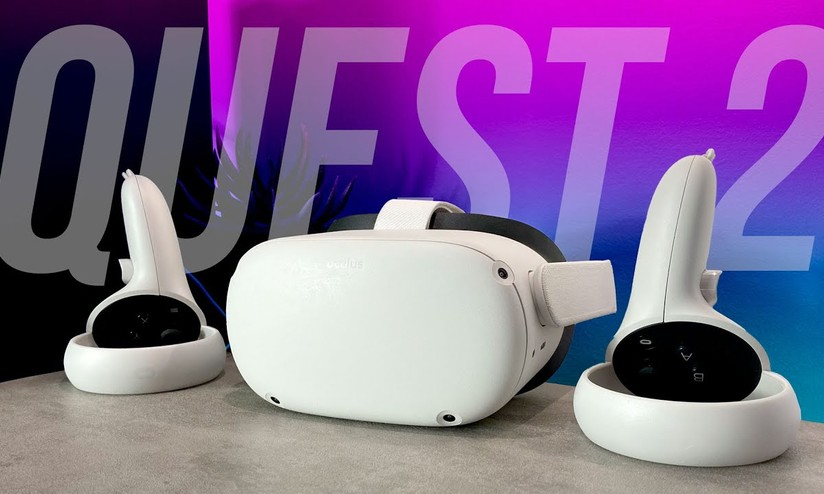
\includegraphics[scale = 0.5]{Immagini/Oculus-Quest-2.jpg}
    \caption{Oculus Quest 2 con i relativi controller}
    \label{fig:Figura 3.1}
\end{figure}
Un \textit{Virtual Reality Headset}\cite{Vrheadset}, o \textit{VR Headset}, è un dispositivo elettronico, detto visore, che permette la visone di applicazioni sviluppate per la Realtà Virtuale.\\Esistono due categorie di \textit{VR Headset}, quelli che necessitano di un collegamento ad un dispositivo Desktop e i dispositivi portatili con hardware dedicato.\\I primi sono i più indicati per lo sviluppo di ambienti in Realtà Virtuale sofisticati, visto che un PC è dotato di una potenza di calcolo mediamente superiore a quella di un dispositivo con hardware dedicato, ma di fatto ciò che l'utente vede è un semplice \gls{render} in tempo reale del mondo virtuale.\\I \textit{VR Headset} portatili con hardware integrato, o \textit{standalone} non offrono una resa grafica alla pari dei visori descritti precedentemente, ma permettono comunque di immergere l'utente in un'ambientazione verosimile, garantendo il vantaggio della portabilità.
\\Il prototipo sviluppato è stato pensato per essere utilizzabile sul modello di visore rappresentato nella \textbf{Figura \ref{fig:Figura 3.1}}.
\\L'Oculus Quest 2 è un modello di visore \textit{standalone}, con esso è possibile non solo giocare ai giochi appositamente pensati per la Realtà Virtuale, ma anche guardare film come se si fosse al cinema, crearsi la propria configurazione multi-monitor per lavorare, visualizzare foto e video a 360 gradi, e fare tutto quello che ci viene in mente sempre immersi in un mondo virtuale.
\\Il visore si può configurare attraverso \textit{l'app Oculus}, scaricabile nel proprio \textit{smartphone}, e, una volta indossato, ci ritroveremo subito all'interno della \textit{home}, dalla quale potremo avviare tutte le \textit{app} e i giochi in nostro possesso. 
\\Nel mondo virtuale si può interagire con i \textit{controller} \textit{Oculus Touch}, le funzionalità pensate per gli utenti in questo prototipo si basano, perciò, sulle specifiche tecniche di questi \textit{controller}.
\section{Unity}
\begin{figure}[H]
    \centering
    
\includegraphics[scale = 0.2]{Immagini/ogimg.jpg}
    \caption{Logo di Unity}
    \label{fig:my_label}
\end{figure} 
\textbf{\textit{Unity}}\cite{unity} è un motore grafico per lo sviluppo di applicazioni 3D e 2D, anche in Realtà Virtuale, nato nel 2005.\\La progettazione di applicazioni è basata sul linguaggio di programmazione C\#(\textit{C sharp}), i cui \textit{\gls{script}} vengono gestiti tramite il software Microsoft Visual Studio.\\L'Editor di \textit{Unity} è supportato da Windows, MacOS e Linux, inoltre le applicazioni che si possono sviluppare sono supportate da piattaforme di vario tipo per esempio:
\begin{itemize}
    \item Mobili: IOS, Android;
    \item Desktop: Windows, MacOS, Linux;
    \item Web: WEBGL;
    \item Console: XBOX, Playstation(PS4, PS5), Nintendo Switch;
    \item Virtual Reality/Extended Reality: Oculus, PlayStation VR, Google's ARCore, Apple's ARKit, Windows Mixed Reality, Google Cardboard.
\end{itemize}
\subsection{Interfaccia Utente}
\begin{figure}[H]
    \centering
    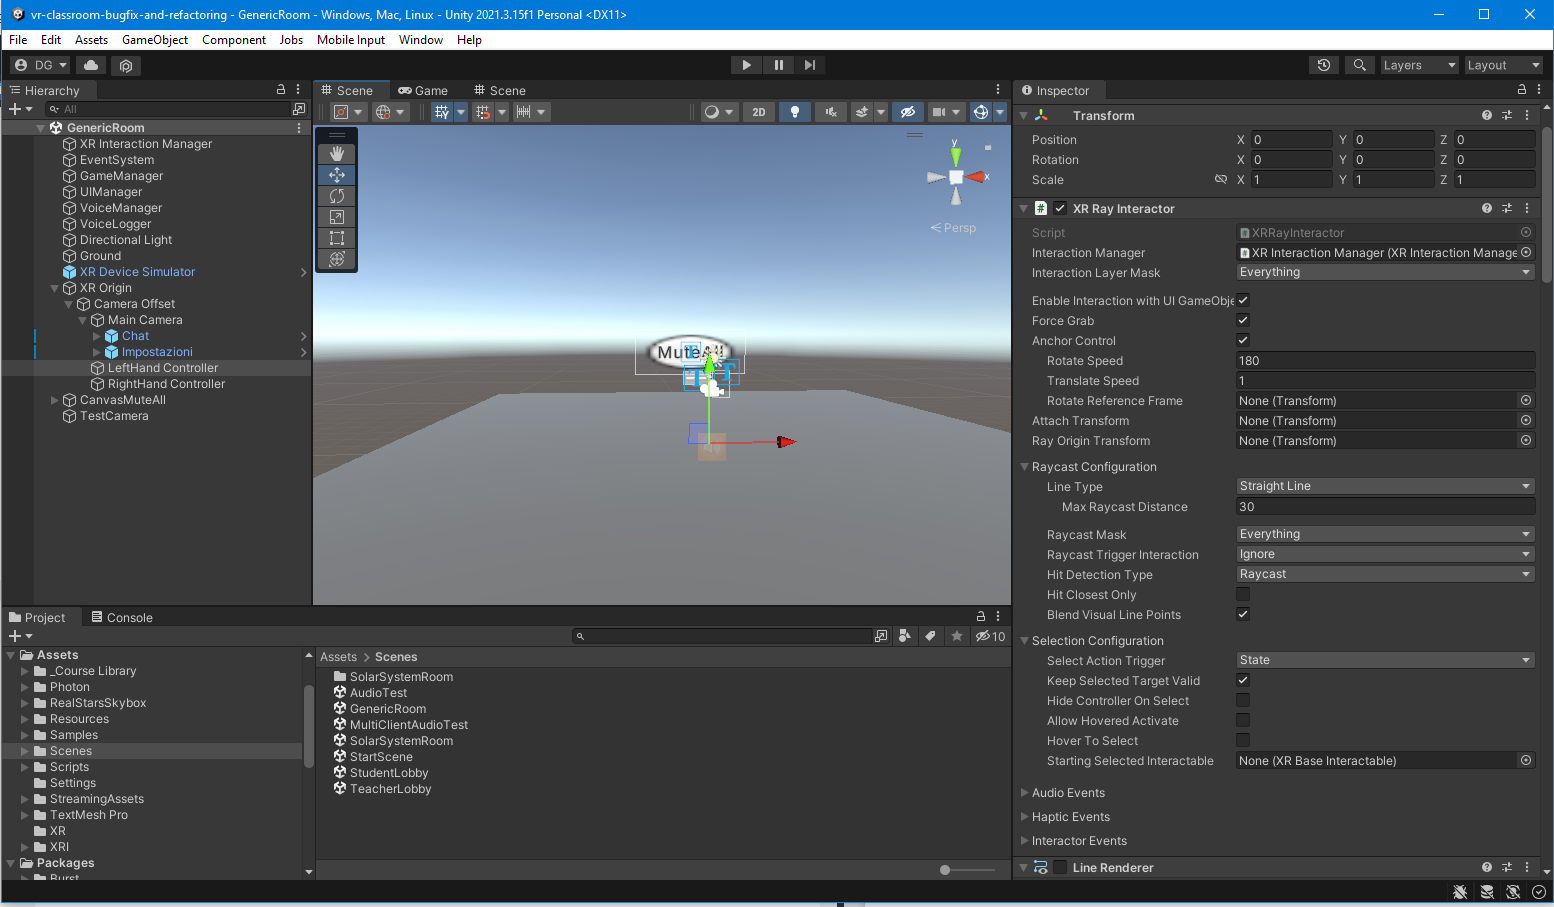
\includegraphics[scale = 0.35]{Immagini/UnityInteface.jpg}
    \caption{Interfaccia utente di Unity 2021.3.15f1}
    \label{fig:my_label}
\end{figure}
L'interfaccia utente\cite{unityMain} di \textit{Unity}, detta anche Unity Editor, è composta da 5 sezioni principali: Hierarchy, Game and Scene, Inspector, Project e Console.
\subsubsection{Hierarchy}
\begin{figure}[H]
    \centering
    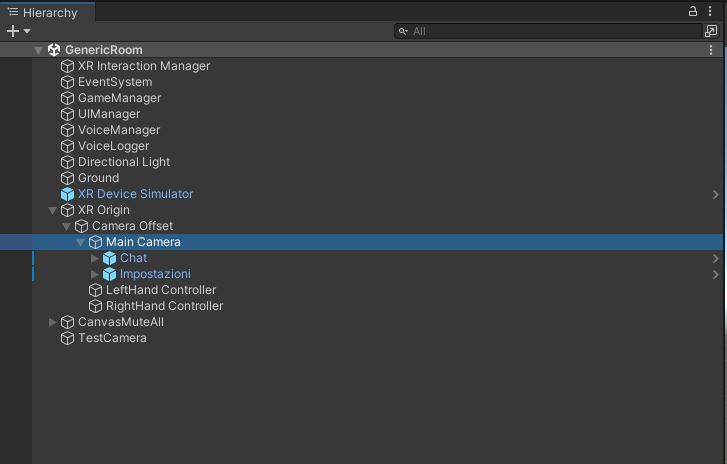
\includegraphics[width=12cm, height=9cm]{Immagini/Hierarchy.jpg}
    \caption{Hierarchy Panel di Unity Editor}
    \label{fig:my_label}
\end{figure}
La Hierarchy\cite{unityhierarchy} è la sezione dell'Editor in cui sono elencati tutti gli oggetti della scena e la relazione che c'è tra essi.\\La relazione tra oggetti è denominata gerarchia, o parentela, ovvero un oggetto può essere un `genitore` o `figlio` di un altro oggetto.\\È lo stesso tipo di relazione si può trovare tra cartelle nel \gls{File System} di un sistema operativo.\\L'oggetto principale, il genitore, trasmette le proprie componenti e proprietà agli oggetti figli, quindi ogni modifica effettuata sull'oggetto genitore verrà applicata anche all'oggetto figlio.\\La relazione di parentela può anche essere presente su più livelli, ossia un oggetto figlio può avere un oggetto figlio e così via.
\subsubsection{Game and Scene}
La Scena\cite{unityScene} è la sezione dell'Editor che rappresenta l'ambiente applicativo vero e proprio, in essa, infatti, sono visibili gli oggetti, detti \textit{GameObject}, che sono stati creati dal programmatore.\\Nella Scena, inoltre, si ha una visione interattiva dell'ambiente applicativo, ovvero è possibile posizionare, selezionare e manipolare gli oggetti.
\\Gli oggetti di scena possono essere di vario tipo per esempio: modelli 3D come cubi e sfere, modelli dotati di \textit{texture}, \textit{controller} per il giocatore, luci per l'ambientazione e una telecamera per rendere visibili tutti gli oggetti della scena, oltre alla scena stessa, nell'applicazione finale.
\\Dalla Scena si può entrare nella Game Mode\cite{unityGame}, quella sezione dell'Editor in cui è possibile testare ciò che si è creato nella Scena, come ad esempio i movimenti del giocatore e dei vari oggetti implementati nella Hierarchy.
\begin{figure}[H]
    \centering
    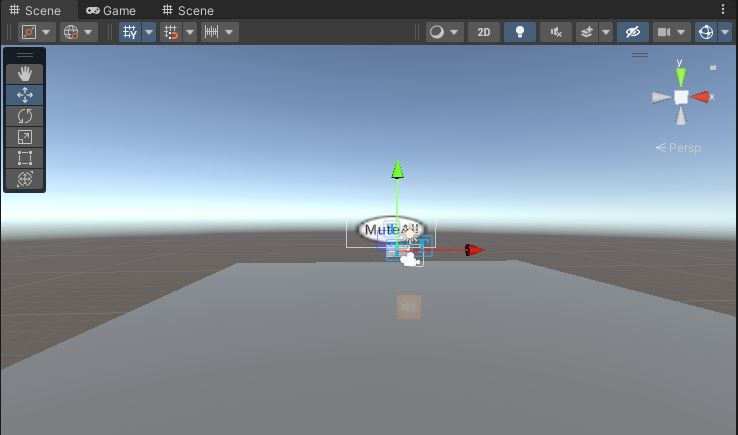
\includegraphics[scale = 0.6]{Immagini/Cattura.jpg}
    \caption{Game and Scene Panel di Unity Editor}
    \label{fig:my_label}
\end{figure}
\subsubsection{Inspector}
L'Inspector\cite{unityInspector} è la sezione dell'Editor dedicata alla gestione delle componenti degli oggetti \textit{Unity}, che possono essere di vario tipo, per esempio: script C\#, Transform, Text, Audio, Video ecc...
\\Sono le componenti dell'oggetto che determinano le funzionalità che ha all'interno della scena, per cui è essenziale applicare le componenti giuste agli oggetti per potergli permettere di compiere le azioni desiderate.
\\Ogni componente possiede dei parametri, che variano a seconda del tipo di componente, che posso essere modificati con mouse e tastiera tramite l'interfaccia utente.
\vspace*{0.5cm}
\begin{figure}[H]
    \centering
    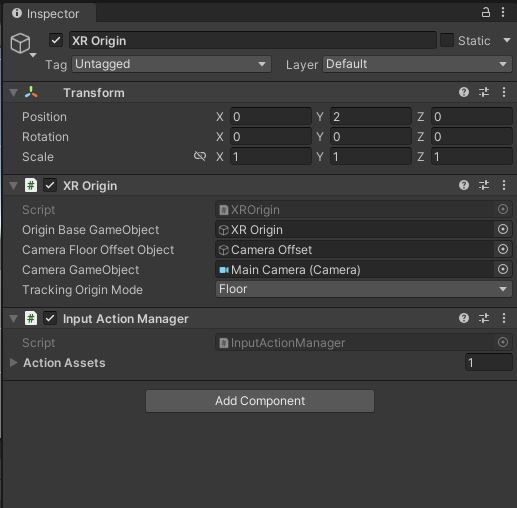
\includegraphics[scale = 1]{Immagini/Inspector.jpg}
    \caption{Inspector Panel di Unity Editor}
    \label{fig:my_label}
\end{figure}
\hspace{-0.6cm}È questo uno dei vantaggi che si ha nello sviluppo di applicazioni con \textit{Unity}, ovvero avere un'interfaccia interattiva nella quale si possono effettuare modifiche su oggetti e componenti che hanno effetto immediato sulla Scena.
\vspace{-2cm}
\subsubsection{Project}
Project\cite{unityProject} è la sezione dell'Editor che mostra la cartella \textit{`Assets`} del progetto creato, che contiene tutti gli elementi che possono essere utilizzati all'interno del progetto.
\\Oltre agli elementi che si possono creare con \textit{Unity}, è possibile creare e importare elementi dell'Assets dall'esterno, come per esempio modelli 3D, file Audio, file Video, immagini o qualsiasi altro file compatibile con \textit{Unity}.
\vspace{1cm}
\begin{figure}[H]
    \centering
    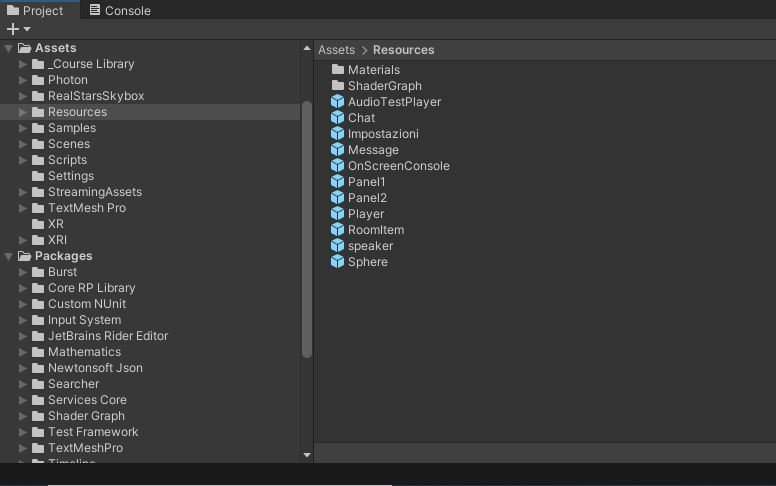
\includegraphics[scale = 0.7]{Immagini/Project.jpg}
    \caption{Project Panel di Unity Editor}
    \label{fig:my_label}
\end{figure}
\subsubsection{Console}
La Console\cite{unityconsole} è la sezione dell'Editor in cui si possono trovare i messaggi di errore, con il simbolo rosso, messaggi di avvertimento (\textit{Warning}) e altri messaggi generati da \textit{Unity}.
\begin{figure}[H]
    \centering
    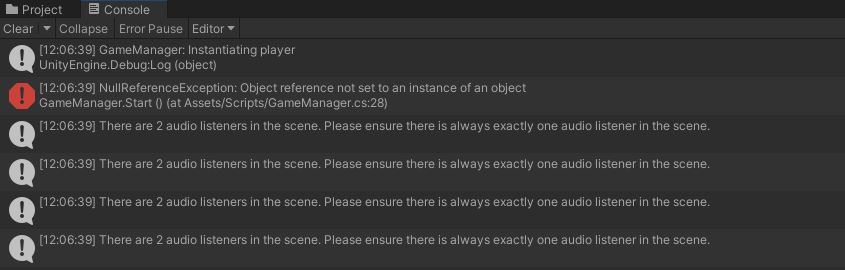
\includegraphics[scale = 0.75]{Immagini/Console.jpg}
    \caption{Console Panel di Unity Editor}
    \label{fig:my_label}
\end{figure}
\hspace{-0.6cm}Si possono anche generare manualmente dei messaggi sulla Console utilizzando i comandi \\\textit{\underline{Debug.Log}}, \textit{\underline{Debug.LogWarning}}, \textit{\underline{Debug.LogError}}.
\section{C\#}
Il C\#\cite{CSharp} è un linguaggio di programmazione multi-paradigma, sviluppato da Microsoft, che supporta tutti i concetti della programmazione orientata agli oggetti, quindi incapsulamento, ereditarietà e polimorfismo.\\La sintassi e la struttura del C\# prendono spunto da vari linguaggi nati precedentemente, in particolare Delphi, C++, Java e Visual Basic.
\subsection{.NET Framework}
I programmi C\# vengono eseguiti su \textit{.NET Framework}\cite{CSharp}, un componente di Windows composto da:
\begin{itemize}
    \item \textit{Common Language Runtime} (CLR);
    \item Librerie di classi di \textit{.NET Framework}.
\end{itemize}
Il \textit{Common Language Runtime} rappresenta la base di \textit{.NET Framework} e può essere considerato come un agente che gestisce il codice in fase di esecuzione (simile alla \textit{Java Virtual Machine}), fornendo servizi di base quali gestione della memoria (\textit{Garbage Collector}), gestione di thread, servizi remoti, networking e attivando una rigida indipendenza dai tipi e altre forme di accuratezza del codice che garantiscono sicurezza ed efficienza.\\Il codice destinato al \textit{runtime} è definito codice gestito, mentre quello non destinato al \textit{runtime} è definito codice non gestito, per esempio una libreria dinamica (DLL) scritta in C/C++.\\Il CLR è responsabile dell'acquisizione del solo codice gestito, della compilazione dello stesso in codice macchina e quindi della sua esecuzione.
\begin{figure}[H]
    \centering
    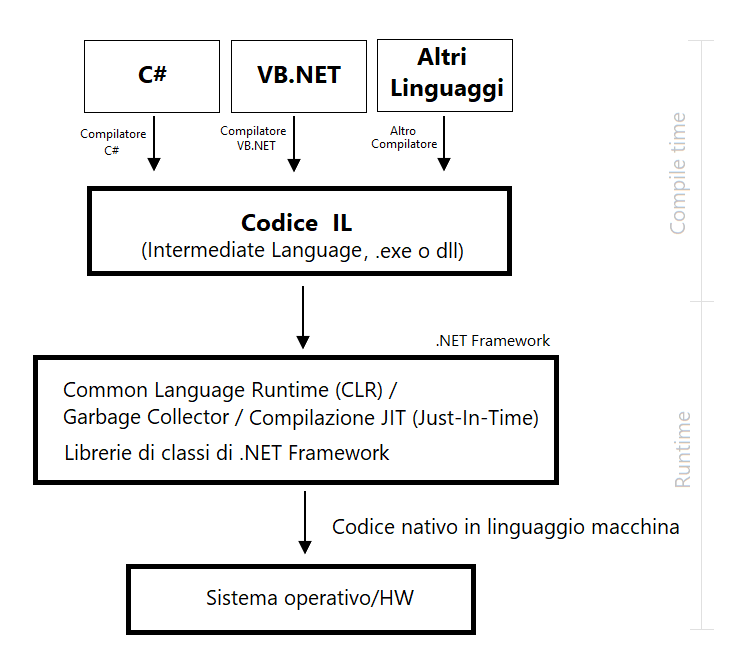
\includegraphics[scale = 0.6]{Immagini/architettura-framework-dotnet.png}
    \caption{Architettura della piattaforma .NET Framework}
    \label{fig:3.9}
\end{figure}
\hspace{-0.6cm}Nella \textbf{Figura \ref{fig:3.9}} sono illustrate le relazioni, in fase di compilazione (\textit{Compile Time}) e di esecuzione (\textit{Runtime}), tra i file di codice sorgente C\#, o degli altri linguaggi, le librerie di classi di \textit{.NET Framework}, gli \textit{assembly} e il CLR.
\\Il codice sorgente scritto in C\# viene compilato in un linguaggio intermedio (\textit{Intermediate Language}, IL). 
\\Il codice IL viene archiviato sul disco in un file eseguibile denominato \textit{assembly}, in genere con estensione EXE o DLL.
\\Quando viene eseguito il programma C\#, l'\textit{assembly} viene caricato nel CLR, e se i requisiti di sicurezza sono soddisfatti, il CLR esegue una compilazione \textit{Just-In-Time} (JIT) per convertire il codice IL in istruzioni del linguaggio macchina nativo.
\\Le librerie di classi sono una raccolta completa e orientata agli oggetti di tipi riusabili, da utilizzare per lo sviluppo di applicazioni, da quelle tradizionali a riga di comando o con interfaccia utente grafica (GUI, \textit{Graphical User Interface}) a quelle basate sulle più recenti innovazioni offerte da ASP.NET, quali Web Form e servizi Web XML, Web API e tanto altro.
\begin{lstlisting}[caption = Esempio di utilizzo di librerie in C\#]
using System.Collections;
using System.Collections.Generic;
using UnityEngine;
...
\end{lstlisting}
\subsection{MonoBehaviour}
\textit{MonoBehaviour}\cite{Mono} è la classe di base che tutti gli script in \textit{Unity} devono avere.\\La classe MonoBehaviour espone una serie di funzioni evento che vengono chiamate da \textit{Unity} al verificarsi di determinate condizioni.
\\Ad esempio, un evento come \textit{MonoBehaviour.OnCollisionEnter()} si verificherà ogni volta che un oggetto entra in collisione con un altro oggetto.
\\Quando questo accade, \textit{Unity} provvederà a richiamare automaticamente il metodo \textit{OnCollisionEnter()}(la lista degli eventi è consultabile qui\cite{Eventi}).
\\Le funzioni evento vanno richiamate all'interno di metodi specifici della classe MonoBehaviour, i 3 principali sono:
\begin{itemize}
    \item \textit{Awake}();
    \item \textit{Start}();
    \item \textit{Update}().
\end{itemize}
I Metodi \textit{\textit{Awake}} e \textit{\textit{Start}} vengono chiamati una sola volta nel ciclo di vita di un oggetto. 
\\La differenza fra i due sta nel fatto che \textit{\textit{Awake}} viene chiamato molto presto, durante la preparazione della scena.
\\In quel momento gli oggetti in scena non sono completamente valorizzati, quindi in \textit{Awake} è sconsigliato svolgere operazioni che richiedono i valori di altri oggetti, come ad esempio leggere il \textit{tag} di un altro oggetto in scena.
\\\textit{\textit{Start}} è utile per eseguire operazioni di preparazione al gioco, come la ricerca di elementi nella scena di cui vogliamo salvare un riferimento per poi lavorarci più avanti durante l'esecuzione.
\\Molto interessante è il tempismo di chiamata dei due metodi a seconda dello stato, attivo o disattivo, dello script in cui compaiono \textit{Awake} e \textit{Start} e il \textit{GameObject} su cui risiede lo script, che viene illustrato nella seguente immagine:
\begin{figure}[H]
    \centering
    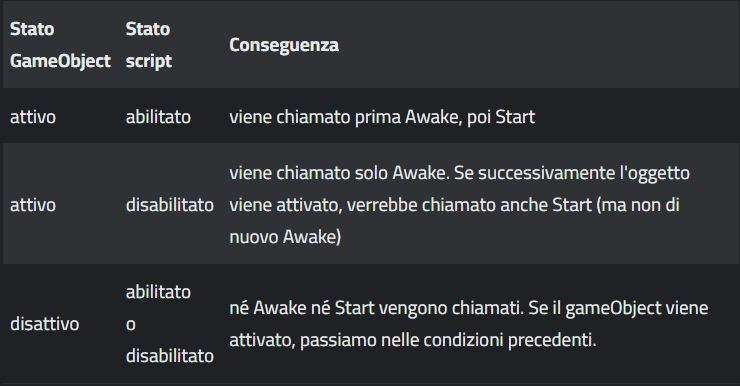
\includegraphics[scale = 0.6]{Immagini/Awake.jpg}]
    \caption{Tempismo di chiamata dei metodi \textit{Awake} e \textit{Start}}
    \label{fig:my_label}
\end{figure} 
\hspace{-0.6cm}Il metodo \textit{Update}, invece, viene chiamato ad ogni frame, il che lo rende molto utile, per esempio, per eseguire azioni come aggiornare o modificare la posizione di oggetti nella scena, per tenere traccia dell'input del giocatore e attribuire comportamenti periodici agli oggetti.
\begin{lstlisting}[language = {[Sharp]C}, caption = {Esempio di utilizzo dei metodi Start e Update}, label{Script}]
using UnityEngine;
using System.Collections;

public class GameObject: MonoBehaviour {

void Start(){ . . . }

void Update(){ . . . }
} 
\end{lstlisting}
\subsection{Librerie Utilizzate}
L'utilizzo di librerie è essenziale per la progettazione e sviluppo di software, sono estremamente utili perché forniscono una collezione di entità di base pronte per l'uso, evitando al programmatore di dover riscrivere ogni volta le stesse funzioni o strutture dati e facilitando così le operazioni di sviluppo e manutenzione.
\\Per la realizzazione di questo prototipo si distinguono in due tipologie di librerie:
\begin{itemize}
    \item Le librerie interne presenti nello \textit{\gls{Unity Registry}};
    \item Le librerie \textit{Photon} importate dall'\textit{\gls{Asset Store}}.
\end{itemize}
\subsubsection{Librerie Interne}
Le principali librerie Interne utilizzate sono:
\begin{itemize}
    \item UnityEngine, raccoglie le classi fondamentali e di riferimento per ogni progetto \textit{Unity}: 
    \begin{itemize}
    \item UnityEngine.Events\cite{UnityEvents};
    \item UnityEngine.InputSystem\cite{UnityInputSystem};
    \item UnityEngine.XR.Interaction.Toolkit\cite{XRToolkit};
    \item UnityEngine.UI\cite{UI}.
    \end{itemize}
    \item{System}, contiene le classi fondamentali e di base che definiscono eventi, gestori di eventi, interfacce, attributi, eccezioni di elaborazione e tipi di dati di riferimento e valore usati comunemente:
    \begin{itemize}
    \item System.Collections\cite{Collection};
    \item System.Collections.Generic\cite{CollectionGeneric}.
    \end{itemize}
    \item TMPro\cite{TMP_pro}, offre soluzioni per il testo relativo all'interfaccia utente dell'applicazione finale.
\end{itemize}
\subsubsection{Librerie Photon}
Le librerie \textit{Photon} importate sono:
\begin{itemize}
    \item Photon.PUN\cite{Photon_PUN};
    \item Photon.Chat\cite{Photon_Chat};
    \item Photon.Voice\cite{Photon_Voice}.
\end{itemize}
\section{Photon Engine}
\begin{figure}[H]
    \centering
    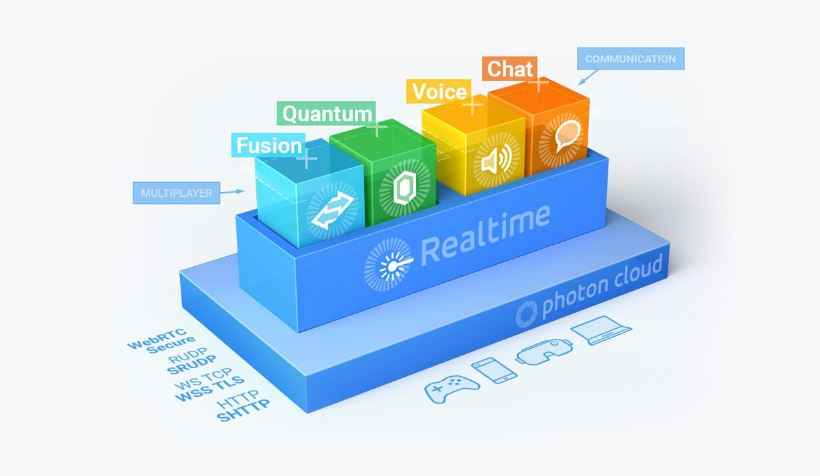
\includegraphics[scale = 0.7]{Immagini/PhotonStructure.jpg}
    \caption{Struttura di Photon Engine}
    \label{fig:3.11}
\end{figure}
\textit{Photon Engine\cite{Photon}} è un motore grafico specializzato nello sviluppo di applicazioni multi-utente.
\\Nella \textbf{Figura \ref{fig:3.11}} si può vedere che il motore grafico è composto da due parti principali:
\begin{itemize}
    \item \textit{Photon Cloud};
    \item \textit{Photon Realtime}.
\end{itemize}
Il \textit{Photon Cloud} è un soluzione \textbf{SaaS} (\textit{Software As A Service}), questo significa che il \textit{\gls{runtime}} locale sul dispositivo client ha già riferimenti al sistema server, che è rilasciato e gestito in un ambiente cloud esterno. \\Il sistema, perciò, non è completamente sotto controllo dell'utente, ma ha dipendenze da componenti remoti di \textit{Photon}.
\\Questo è il motivo principale per cui i servizi offerti da \textit{Photon} sono stati scelti per sviluppare le funzionalità di rete.
\\Il \textit{Photon Realtime} è la parte del motore grafico composta dai \textit{packages} e dalle librerie, quindi sono gli strumenti che l'utente deve utilizzare per sviluppare la propria applicazione multi-utente.
\\In particolare per lo sviluppo del prototipo sono state utilizzate 3 applicazioni del \textit{Photon Realtime}:
\begin{itemize}
    \item PUN (\textit{Photon Unity Networking}), utilizzata per la connessione tra utenti;
    \item \textit{Photon Voice}, utilizzata per la comunicazione vocale tra utenti;
    \item \textit{Photon Chat}, utilizzata per la comunicazione via chat tra utenti.
\end{itemize}
\subsection{Implementazione di PUN in Unity}
In questa sezione saranno illustrati i passaggi fondamentali per la preparazione di un progetto \textit{Unity} alle funzionalità multi-utente di \textit{Photon}.
\begin{figure}[H]
    \centering
    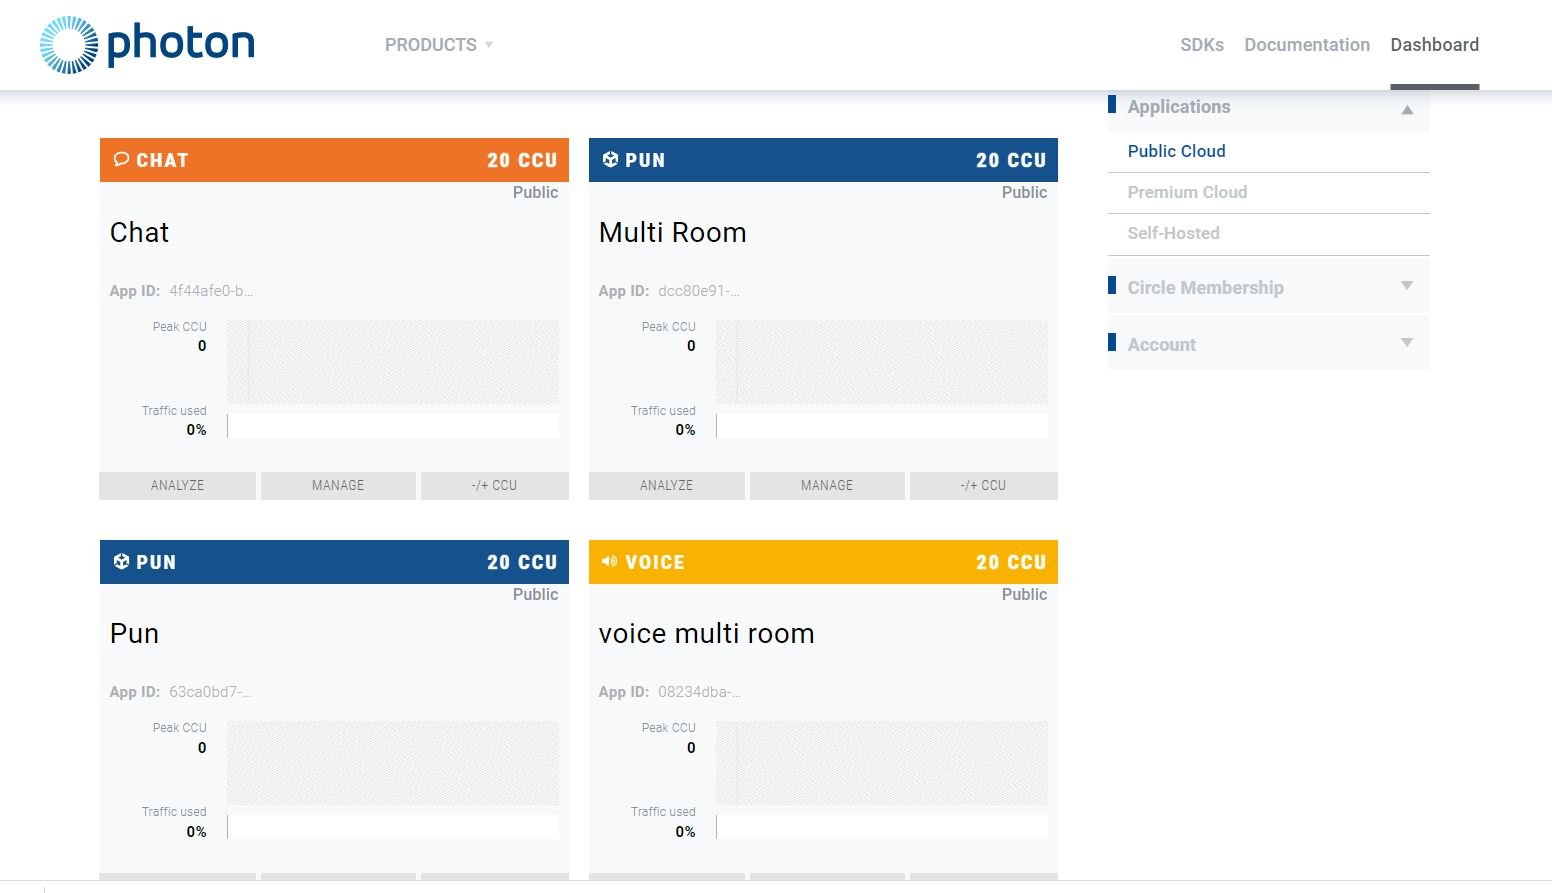
\includegraphics[scale = 0.3]{Immagini/Sitophoton.jpg}
    \caption{Dashboard delle applicazioni Photon Realtime}
    \label{fig:3.12}
\end{figure}
\hspace{-0.6cm}La \textbf{Figura \ref{fig:3.12}} mostra la dashboard delle applicazioni \textit{Photon} Realtime descritte in precedenza, l'accesso alla dashboard è consentito dopo aver creato un account \textit{Photon} gratuitamente.
\\Ogni applicazione, Chat, PUN o Voice, è caratterizzata da un App ID che, dopo aver installato il package PUN
dall'Asset Store di \textit{Unity}, va inserito nell'apposito campo nella sezione dell'editor \textit{`Window/Photon Unity Networking/Highlight Server Settings`}.
\begin{figure}[H]
    \centering
    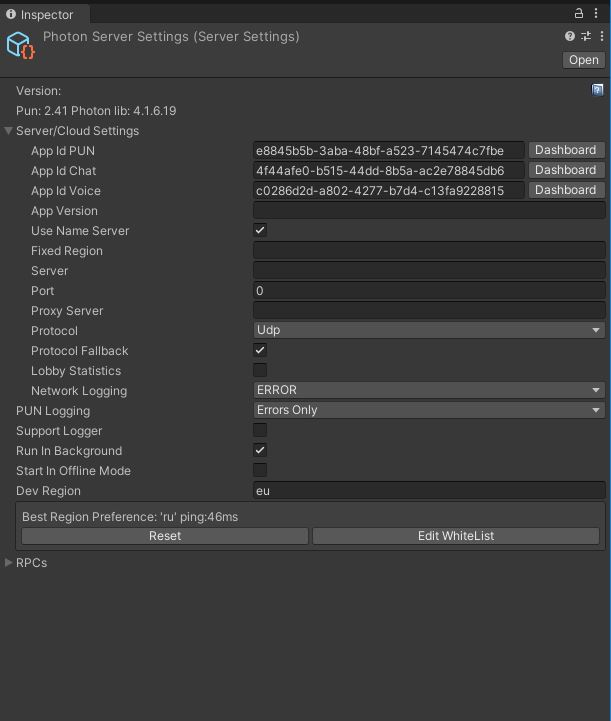
\includegraphics[scale = 0.7]{Immagini/Setting.jpg}
    \caption{Photon Server Settings}
    \label{fig:my_label}
\end{figure}
\hspace{-0.6cm}A questo punto la fase di preparazione del progetto alle funzionalità network è terminata e si può procedere con la progettazione delle funzioni per la connettività tra utenti.
\input{Capitoli/Sviluppo funzionalità}
\chapter{Dimostrazioni d'uso}
In questo capitolo verranno mostrate alcune immagini, dell'applicazione per desktop, che hanno lo scopo di mostrare il funzionamento delle specifiche software che sono state ideate per la realizzazione del prototipo.
\section{Identificazione}
La \textbf{Figura \ref{fig:5.1}} e \textbf{Figura \ref{fig:5.2}} mostrano come il sistema faccia apparire, così come indicato nelle specifiche, un messaggio di errore all'utente quando inserisce delle credenziali errate nei pannelli \textit{username} e \textit{password}.
\begin{figure}[H]
\centering
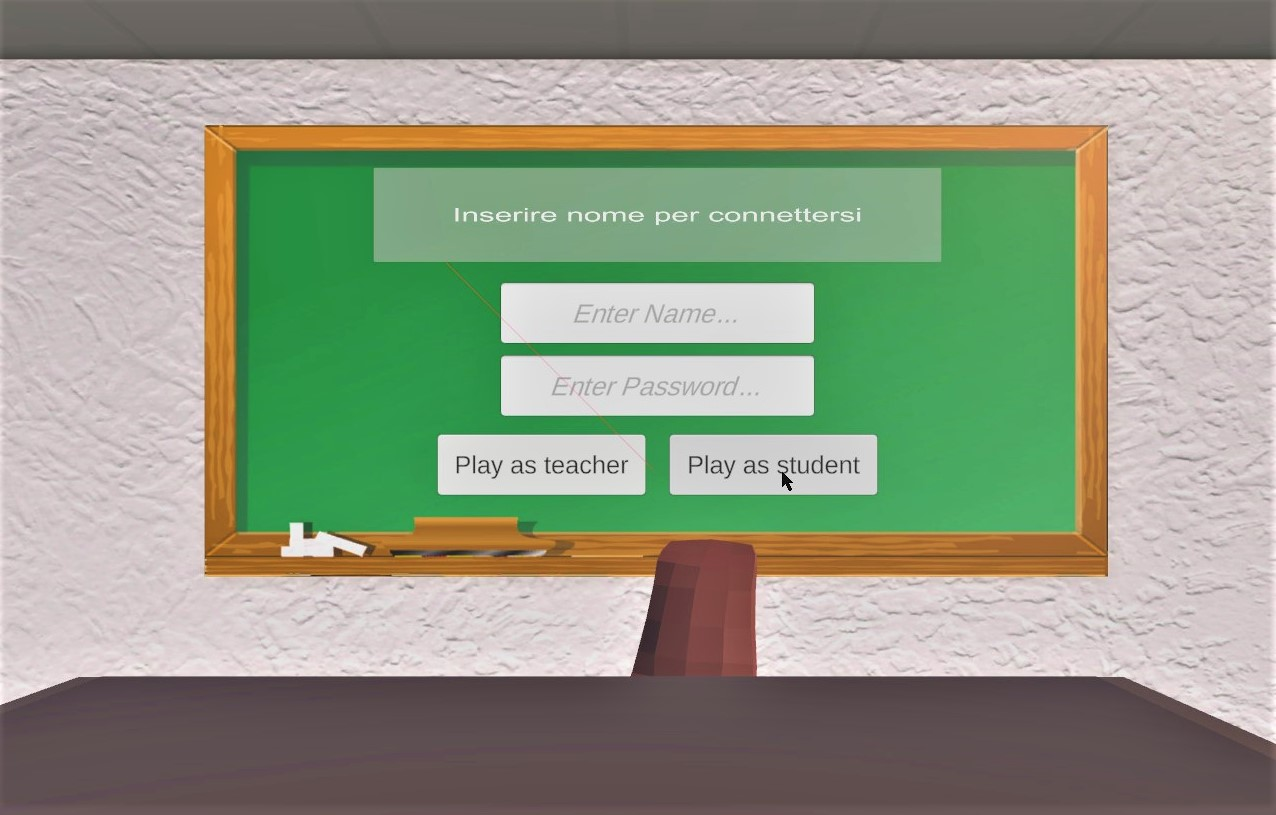
\includegraphics[scale = 0.3]{Immagini/Dimostrazioni d'uso/loginstuderr.jpg}
\caption{Schermata di errore per lo studente}
\label{fig:5.1}
\end{figure}
\begin{figure}[H]
\centering
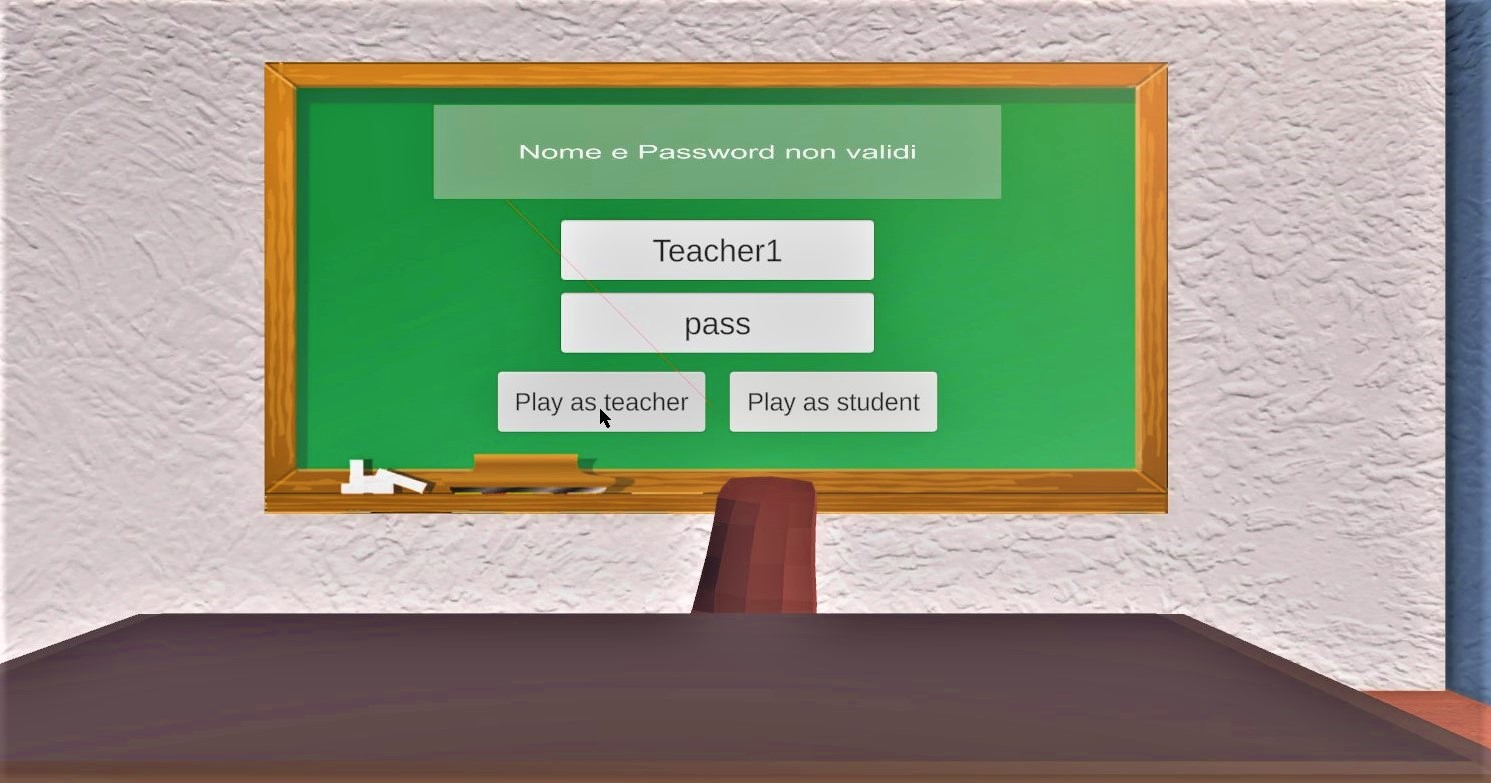
\includegraphics[scale = 0.3]{Immagini/Dimostrazioni d'uso/loginteacherr.jpg}
\caption{Schermata di errore per il docente}
\label{fig:5.2}
\end{figure}
\hspace{-0.6cm}La versione per desktop presenta un problema quando viene eseguita sul visore di riferimento, ovvero l’Oculus Quest 2. 
\\Per delle limitazioni presenti nell'XR Origin, non è possibile utilizzare la tastiera di sistema. 
\\Per ovviare a questo problema, è stato deciso di inserire, nella versione per Oculus Quest 2, un nome di default per gli studenti in modo da poter permettere il login anche tramite visore quando l'utente prova ad accedere senza inserire il nome.
\section{Lobby}
\begin{figure}[H]
\centering
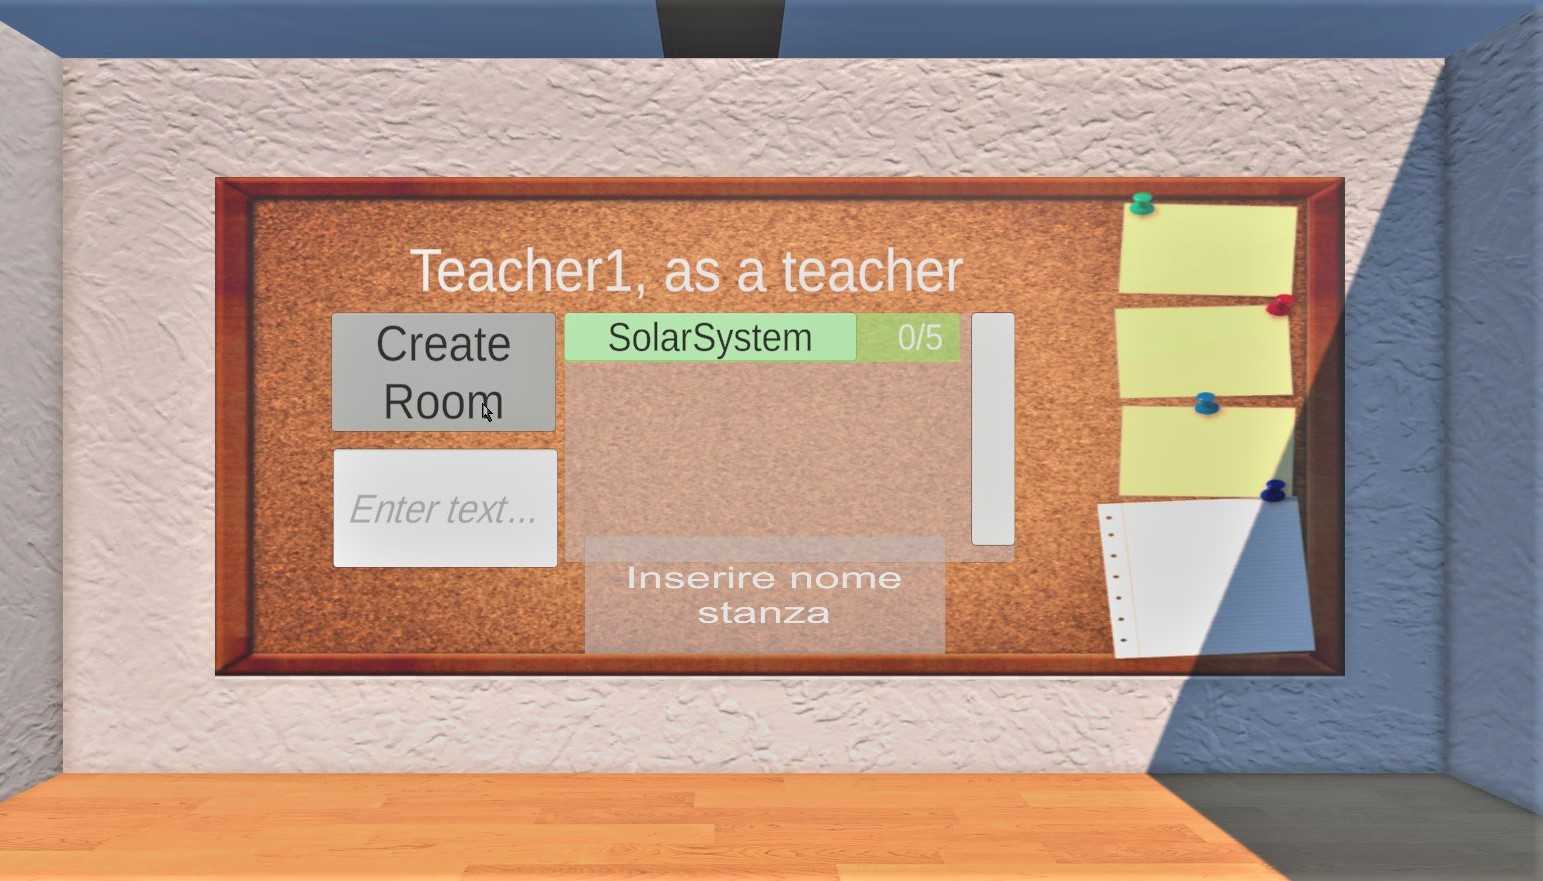
\includegraphics[scale = 0.25]{Immagini/Dimostrazioni d'uso/createroomerr.jpg}
\caption{Lobby docente}
\label{fig:5.3}
\end{figure}
La \textbf{Figura \ref{fig:5.3}} rappresenta la scena che verrà caricata dall'applicazione dell'utente se è stato effettuato l'accesso come docente.
\\Si può notare la presenza del pulsante per creare la stanza (pulsante \textit{Create Room}) e dell'elenco delle stanze disponibili per l'accesso.
\\In particolare, nella figura è presente un messaggio di errore che compare quando il docente cerca di creare una stanza senza nome.
\begin{figure}[H]
\centering
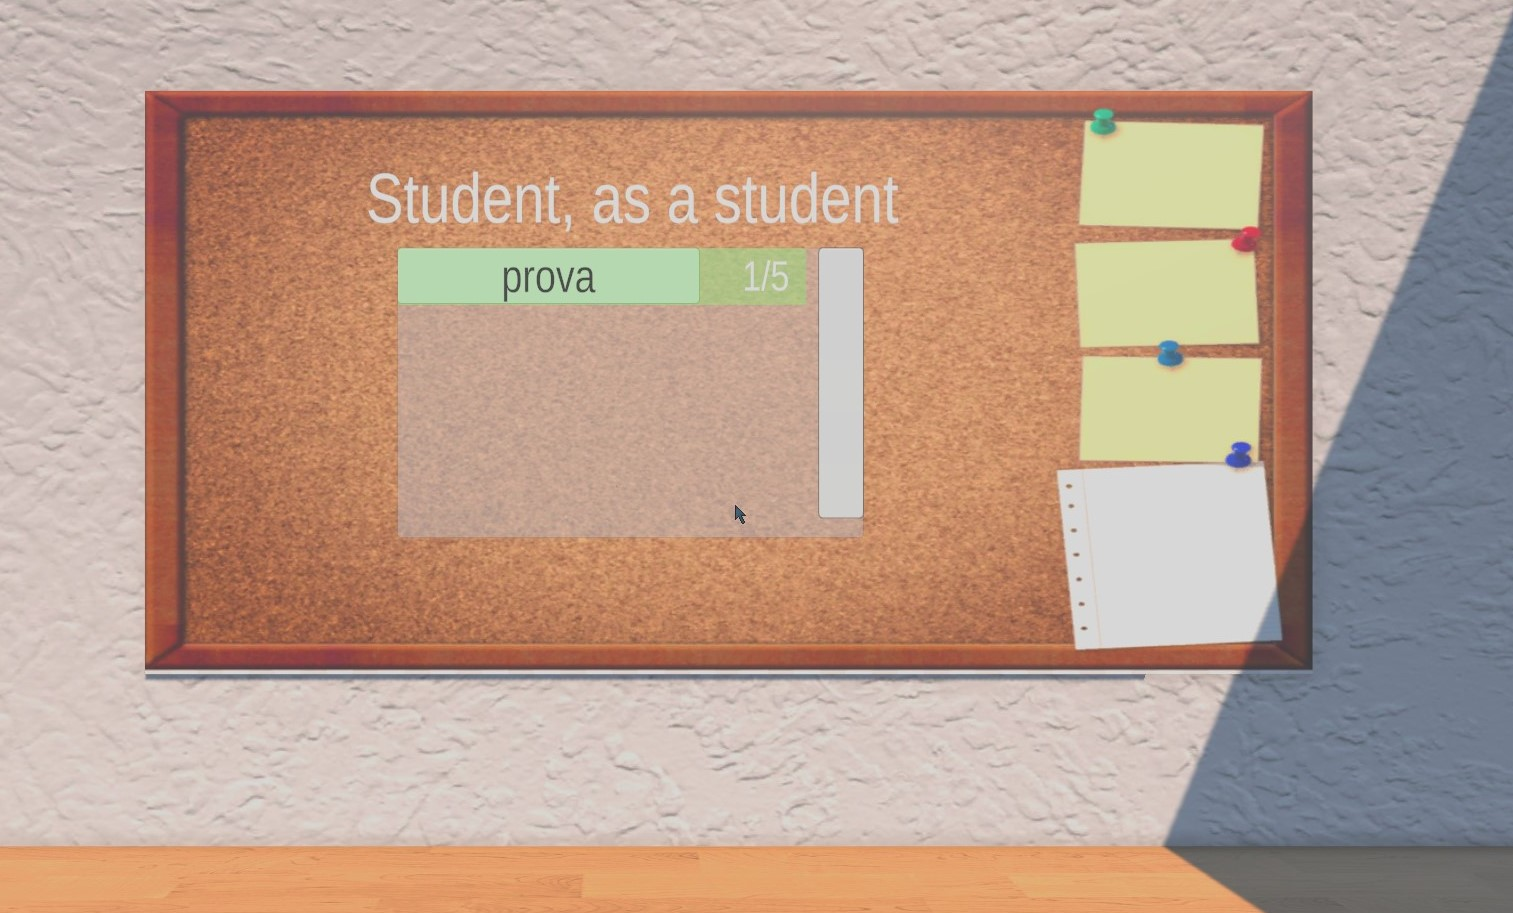
\includegraphics[scale = 0.25]{Immagini/Dimostrazioni d'uso/studlobby.jpg}
\caption{Lobby studente}
\label{fig:5.4}
\end{figure}
\hspace{-0.6cm}La scena rappresentata nella \textbf{Figura \ref{fig:5.4}} è quella caricata dall'applicazione dell'utente se è stato effettuato l'accesso come studente.
\\Lo studente, come già detto nelle specifiche e nei casi d'uso, visualizzerà solo l'elenco delle stanze a cui può unirsi.
\section{Generic Room}
La \textbf{Generic Room} rappresenta la scena del prototipo adibita all'interazione fra gli utenti, ovvero la parte del progetto dove sono implementate le funzionalità descritte nel \textbf{Cap.4}.
\begin{figure}[H]
\centering
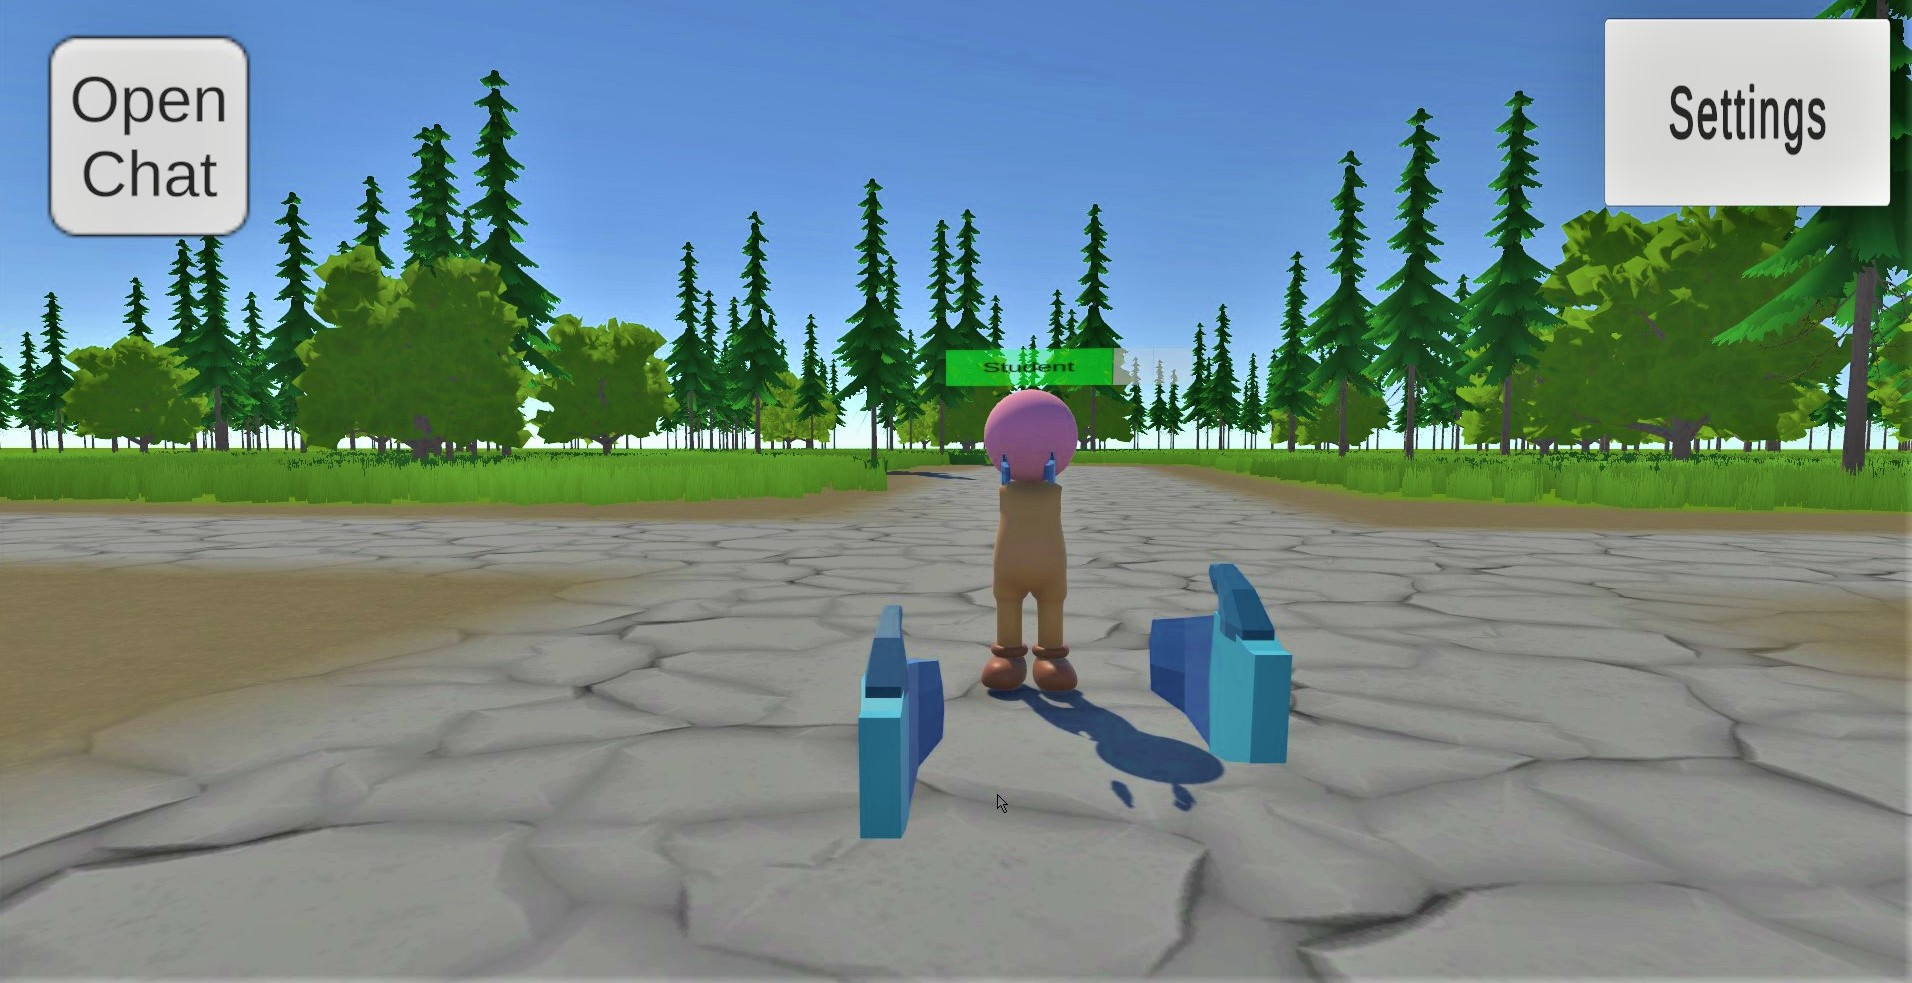
\includegraphics[scale = 0.25]{Immagini/Dimostrazioni d'uso/civediamo.jpg}
\caption{Visualizzazione fra utenti}
\label{fig:5.5}
\end{figure}
\hspace{-0.6cm}Uno dei requisiti fondamentali illustrato nelle specifiche del prototipo è quello della percezione fra utenti.
\\La \textbf{Figura \ref{fig:5.5}} rappresenta la visuale di un utente (\textit{Teacher}), nella quale è ben visibile un secondo utente (\textit{Student}).
\subsection{Chat di testo e Impostazioni}
\begin{figure}[H]
\centering
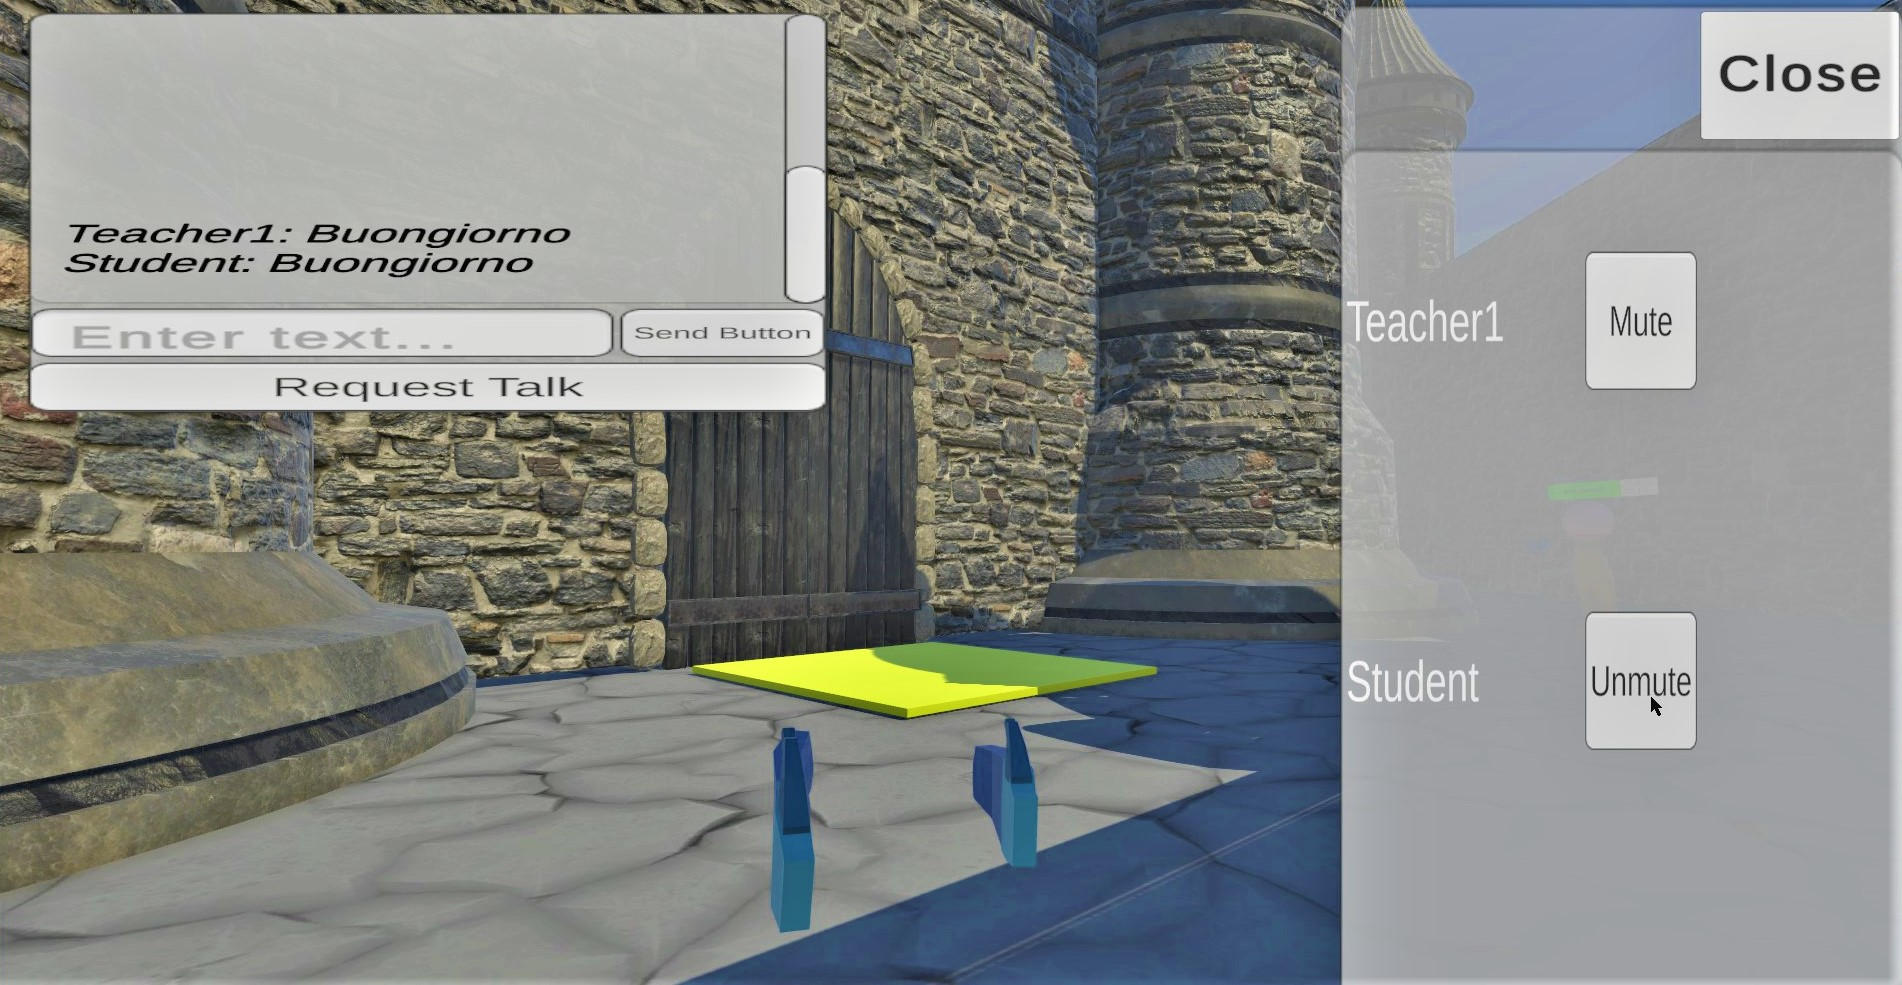
\includegraphics[scale = 0.25]{Immagini/Dimostrazioni d'uso/impostazioni.jpg}
\caption{Funzionamento della Chat e delle Impostazioni}
\label{fig:5.6}
\end{figure}
Nella \textbf{Figura \ref{fig:5.6}} si può notare la presenza della chat sul lato sinistro in cui sono presenti due messaggi, uno inviato dal docente (\textit{Teacher 1}) e uno inviato dallo studente (\textit{Student}).
\\Le impostazioni, che sono accessibili solamente dal docente, si trovano sul lato destro della schermata e, come previsto dai requisti, presentano una lista con i giocatori connessi alla stanza e un bottone per ogni giocatore per l'attivazione o disattivazione del microfono.
\\In particolare, nella figura si nota che il docente ha disattivato il microfono dello studente.
\\La scritta sul bottone accanto al nome dello studente è passata da `Mute` (disattiva il microfono) a `Unmute` (attiva il microfono), se il bottone verrà premuto dal docente, il microfono verrà di nuovo attivato.
\subsection{Creazione/Eliminazione di bandierine}
Le immagini che seguiranno hanno scopo di mostrare sequenzialmente il funzionamento della creazione e distruzione delle bandierine da parte del docente.
\\Saranno presenti immagini sia dal punto di vista del docente sia da quello dello studente, per mostrare in modo ottimale lo svolgimento delle funzionalità.
\\La presenza della chat, nelle suddette immagini, risulta utile per percepire la contemporaneità degli eventi mostrati, infatti sia dal punto di vista dello studente che da quello del docente sono presenti gli stessi messaggi.
\begin{figure}[H]
\centering
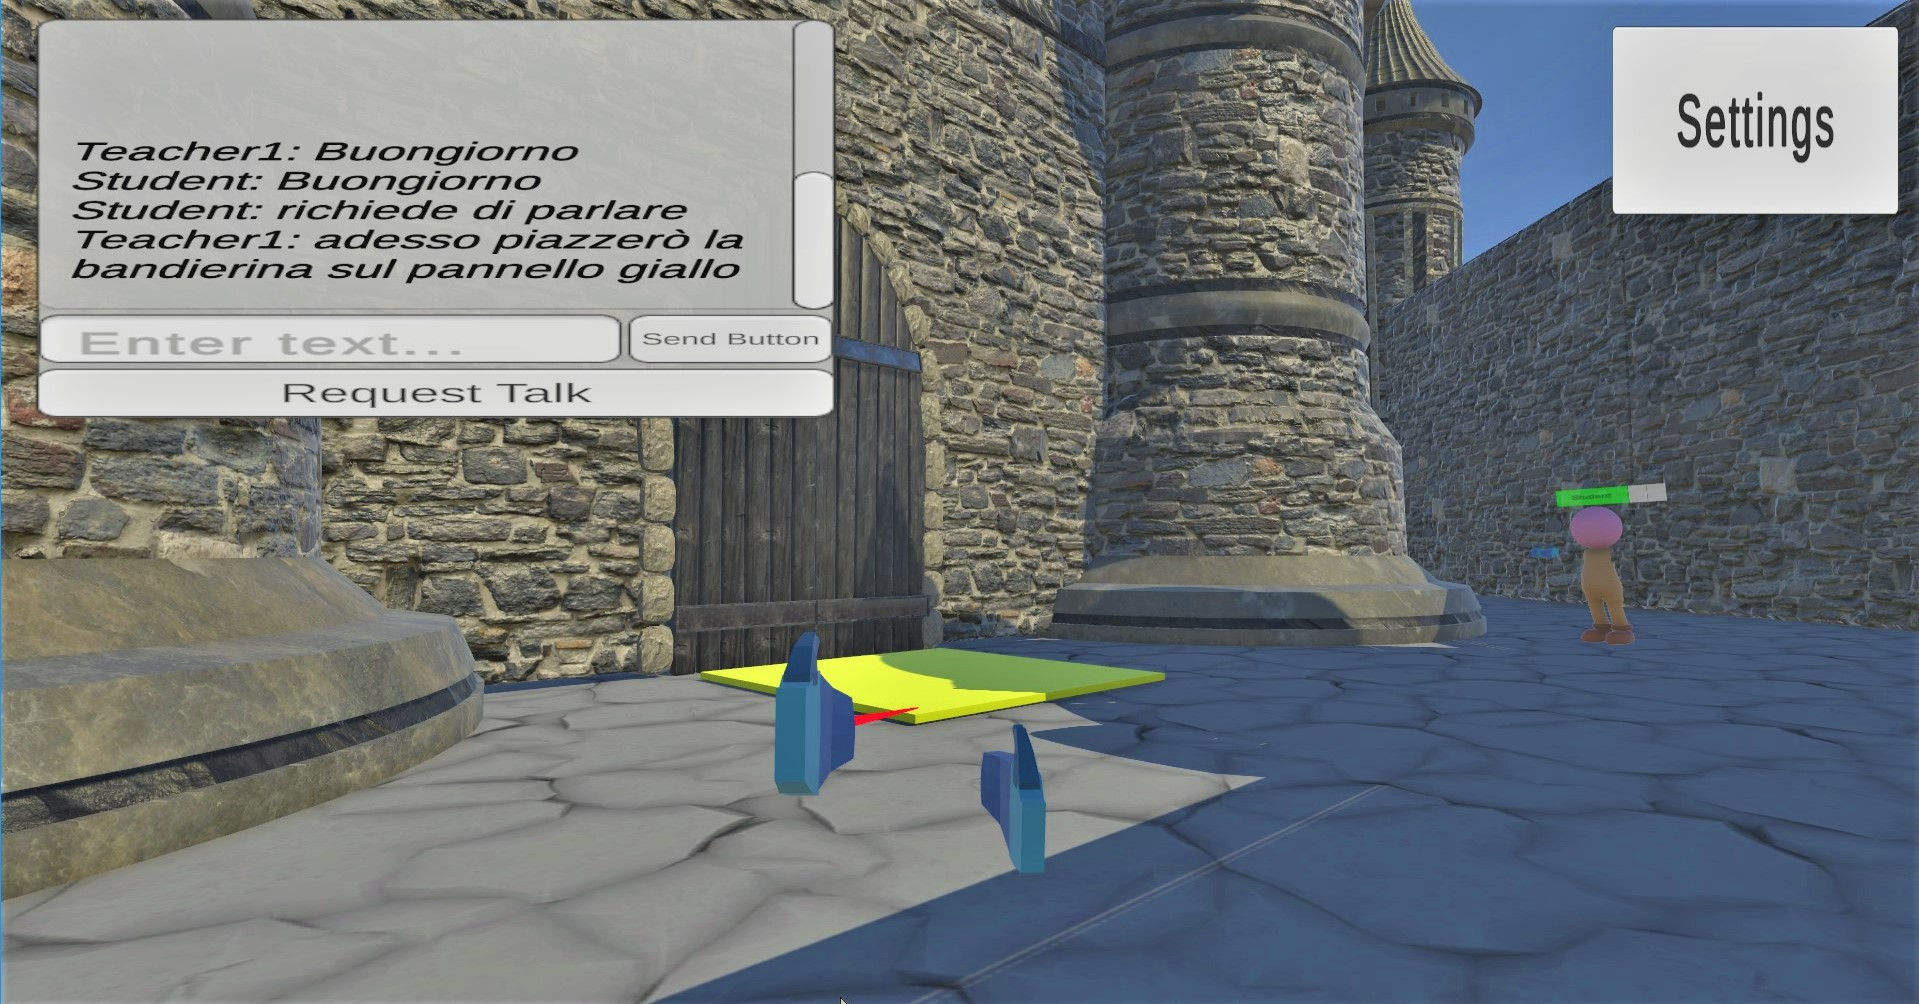
\includegraphics[scale = 0.25]{Immagini/Dimostrazioni d'uso/piazzobandierina.jpg}
\caption{Scena prima del piazzamento della bandierina}
\end{figure}
\begin{figure}[H]
\centering
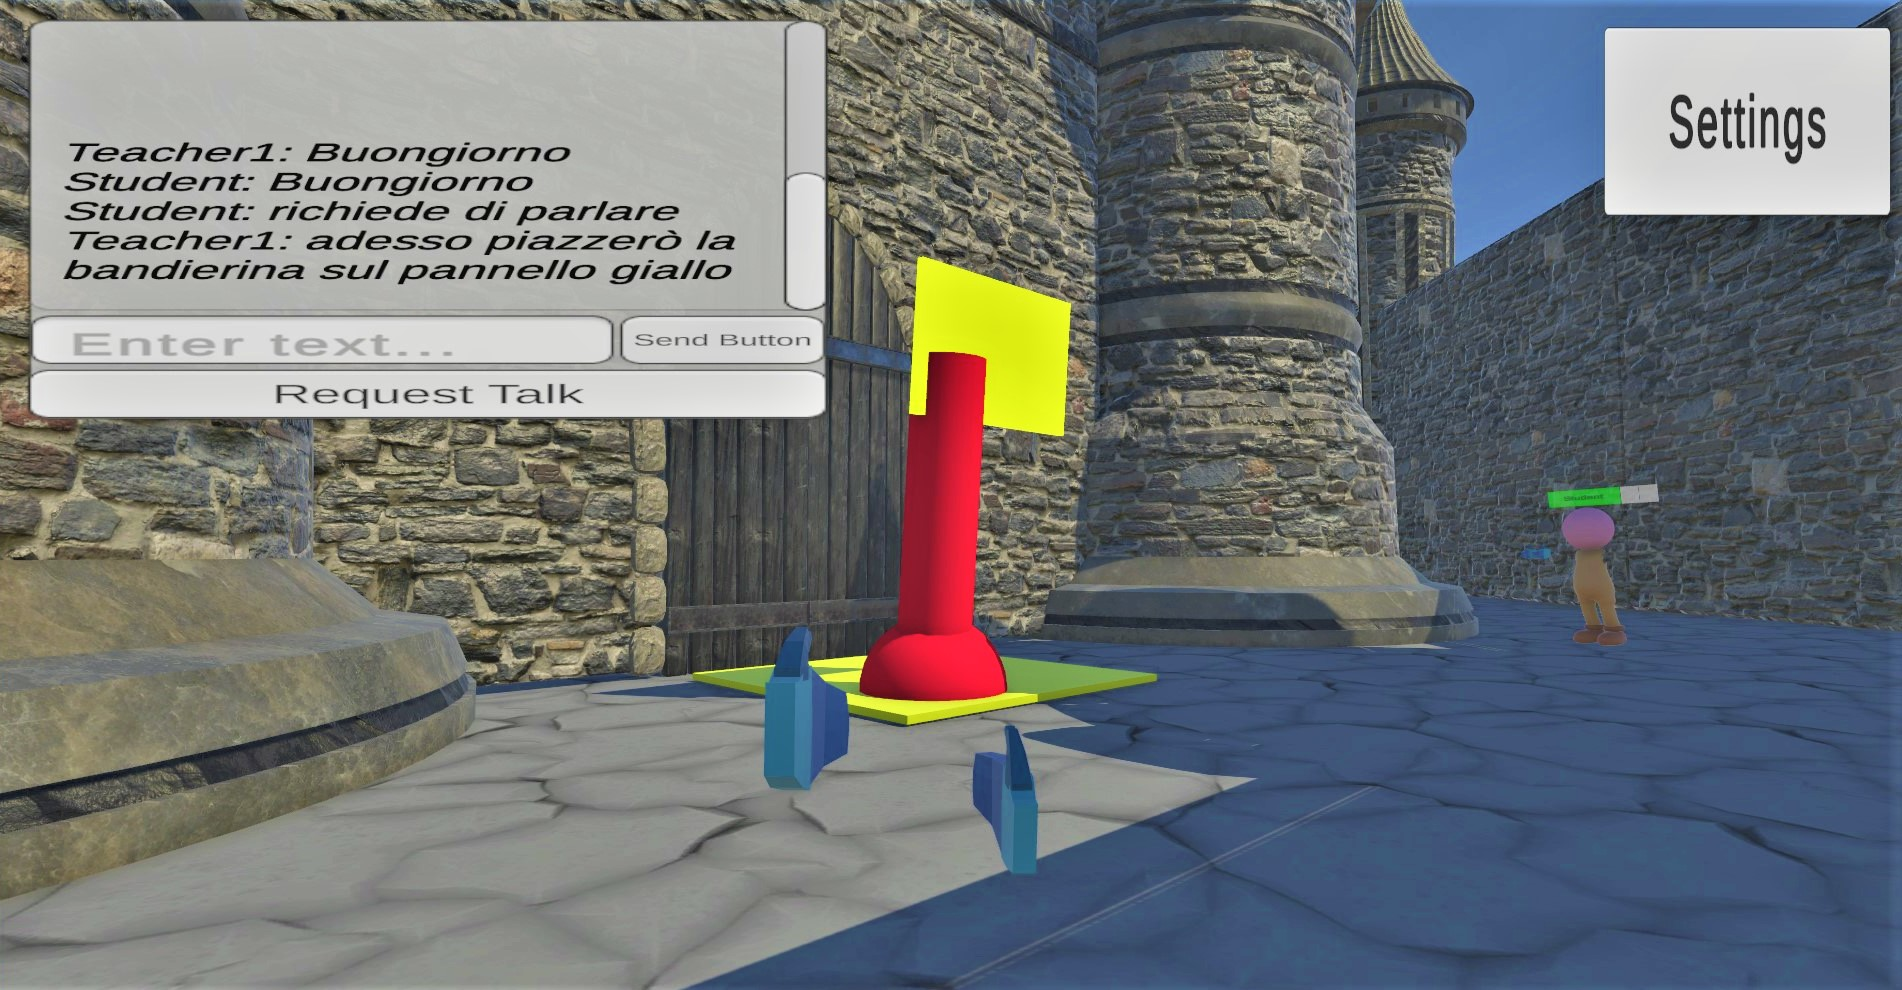
\includegraphics[scale = 0.25]{Immagini/Dimostrazioni d'uso/bandierinapiazzatalatodocente.jpg}
\caption{Scena dopo il piazzamento della bandierina lato docente}
\end{figure}\begin{figure}[H]
\centering
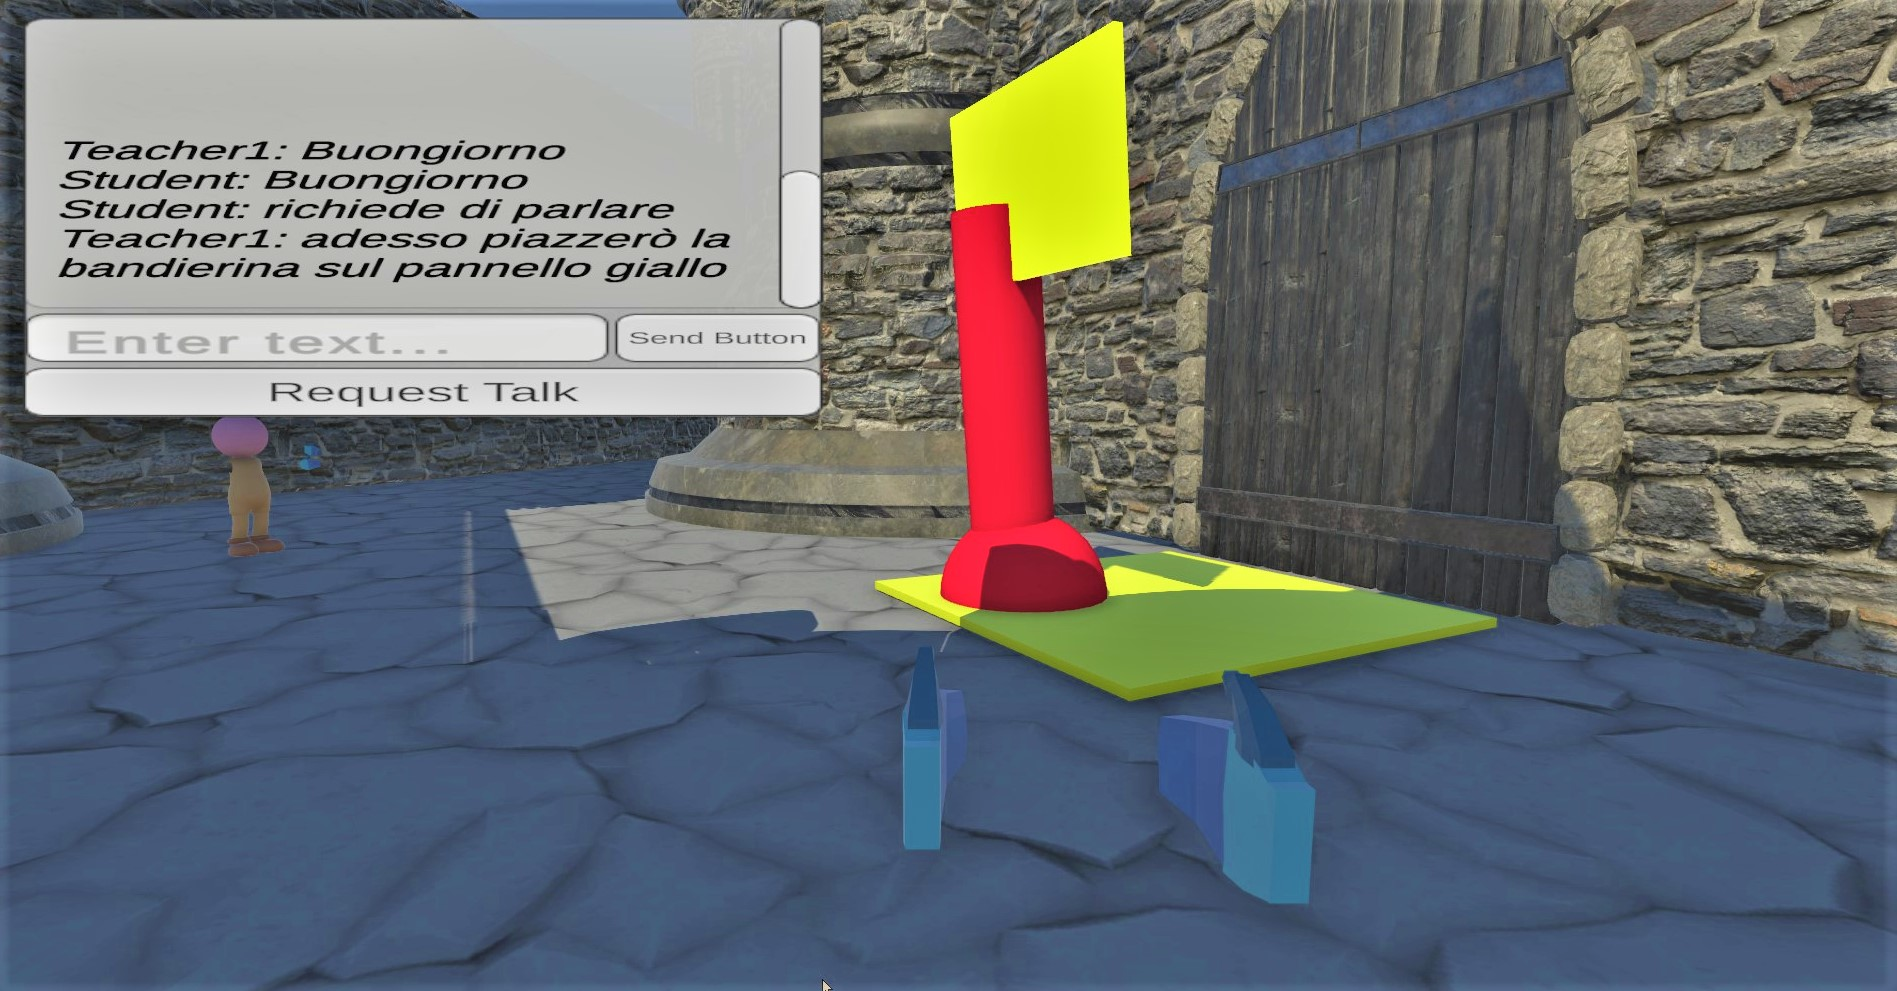
\includegraphics[scale = 0.25]{Immagini/Dimostrazioni d'uso/bandierinapiazzatalatostudente.jpg}
\caption{Scena dopo il piazzamento della bandierina lato studente}
\end{figure}
\begin{figure}[H]
\centering
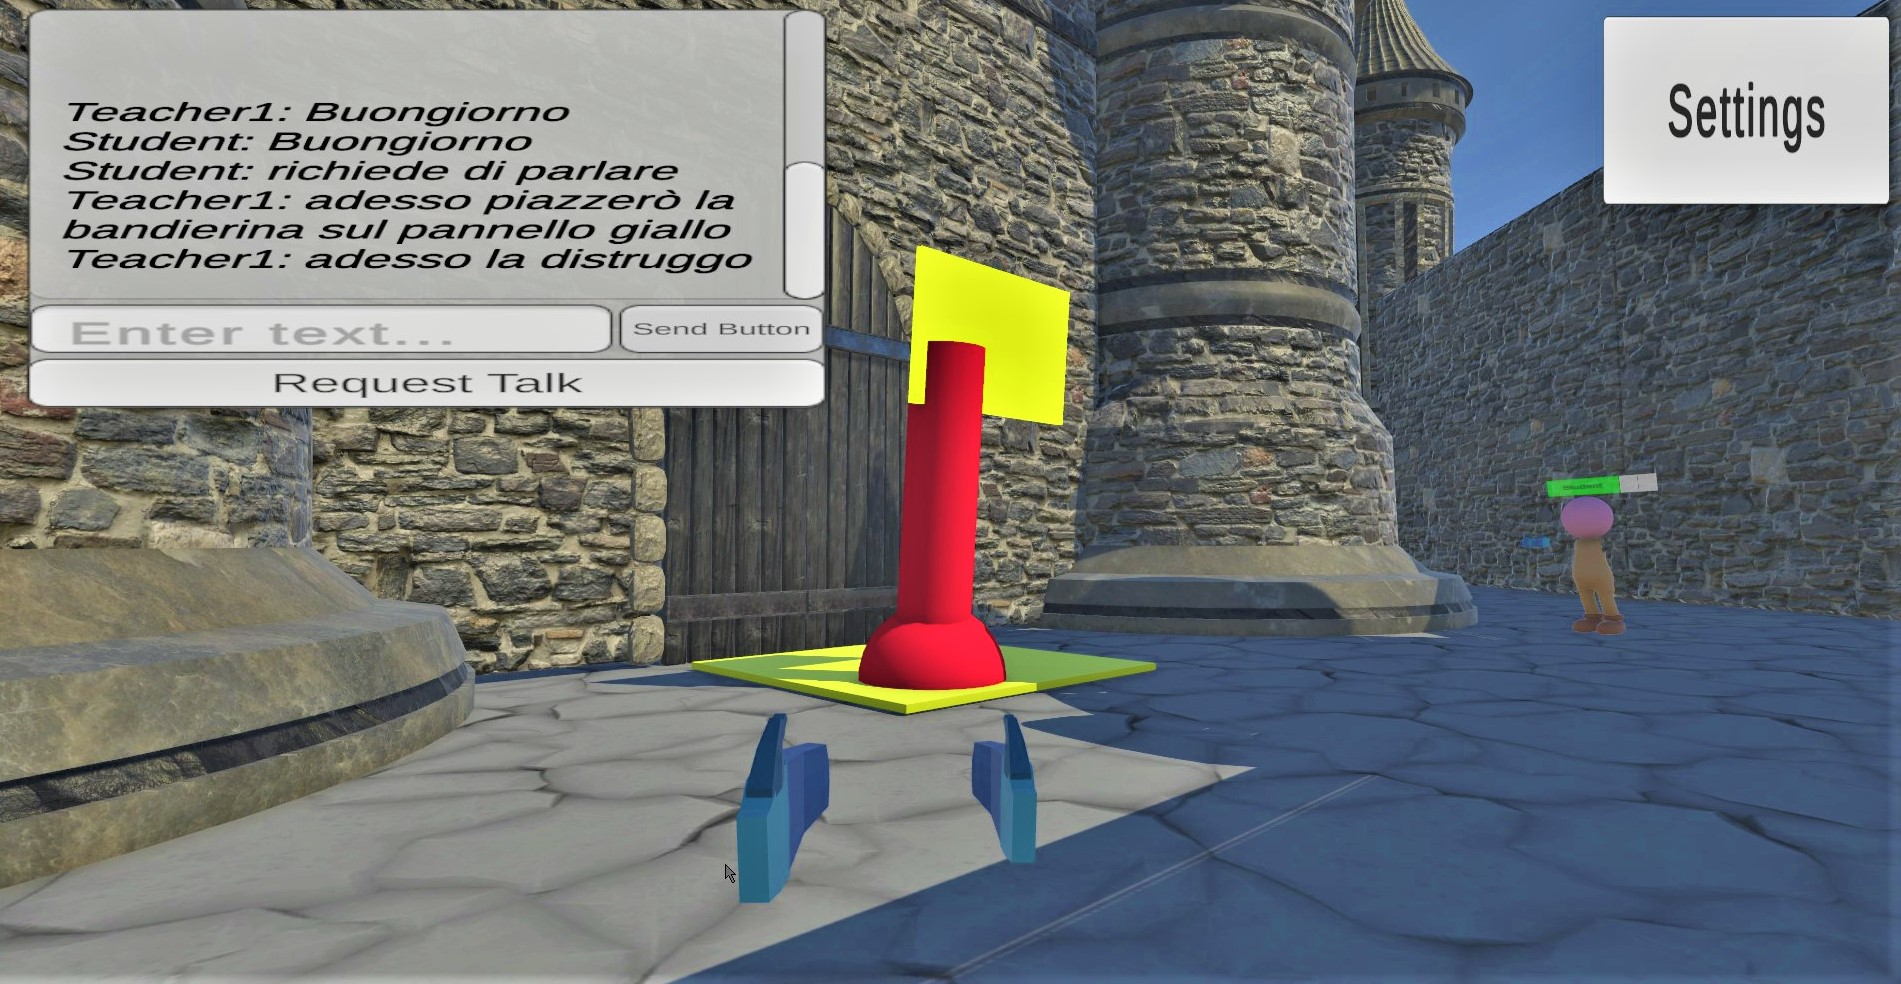
\includegraphics[scale = 0.25]{Immagini/Dimostrazioni d'uso/adessoladistruggo.jpg}
\caption{Scena prima della distruzione della bandierina}
\end{figure}
\begin{figure}[H]
\centering
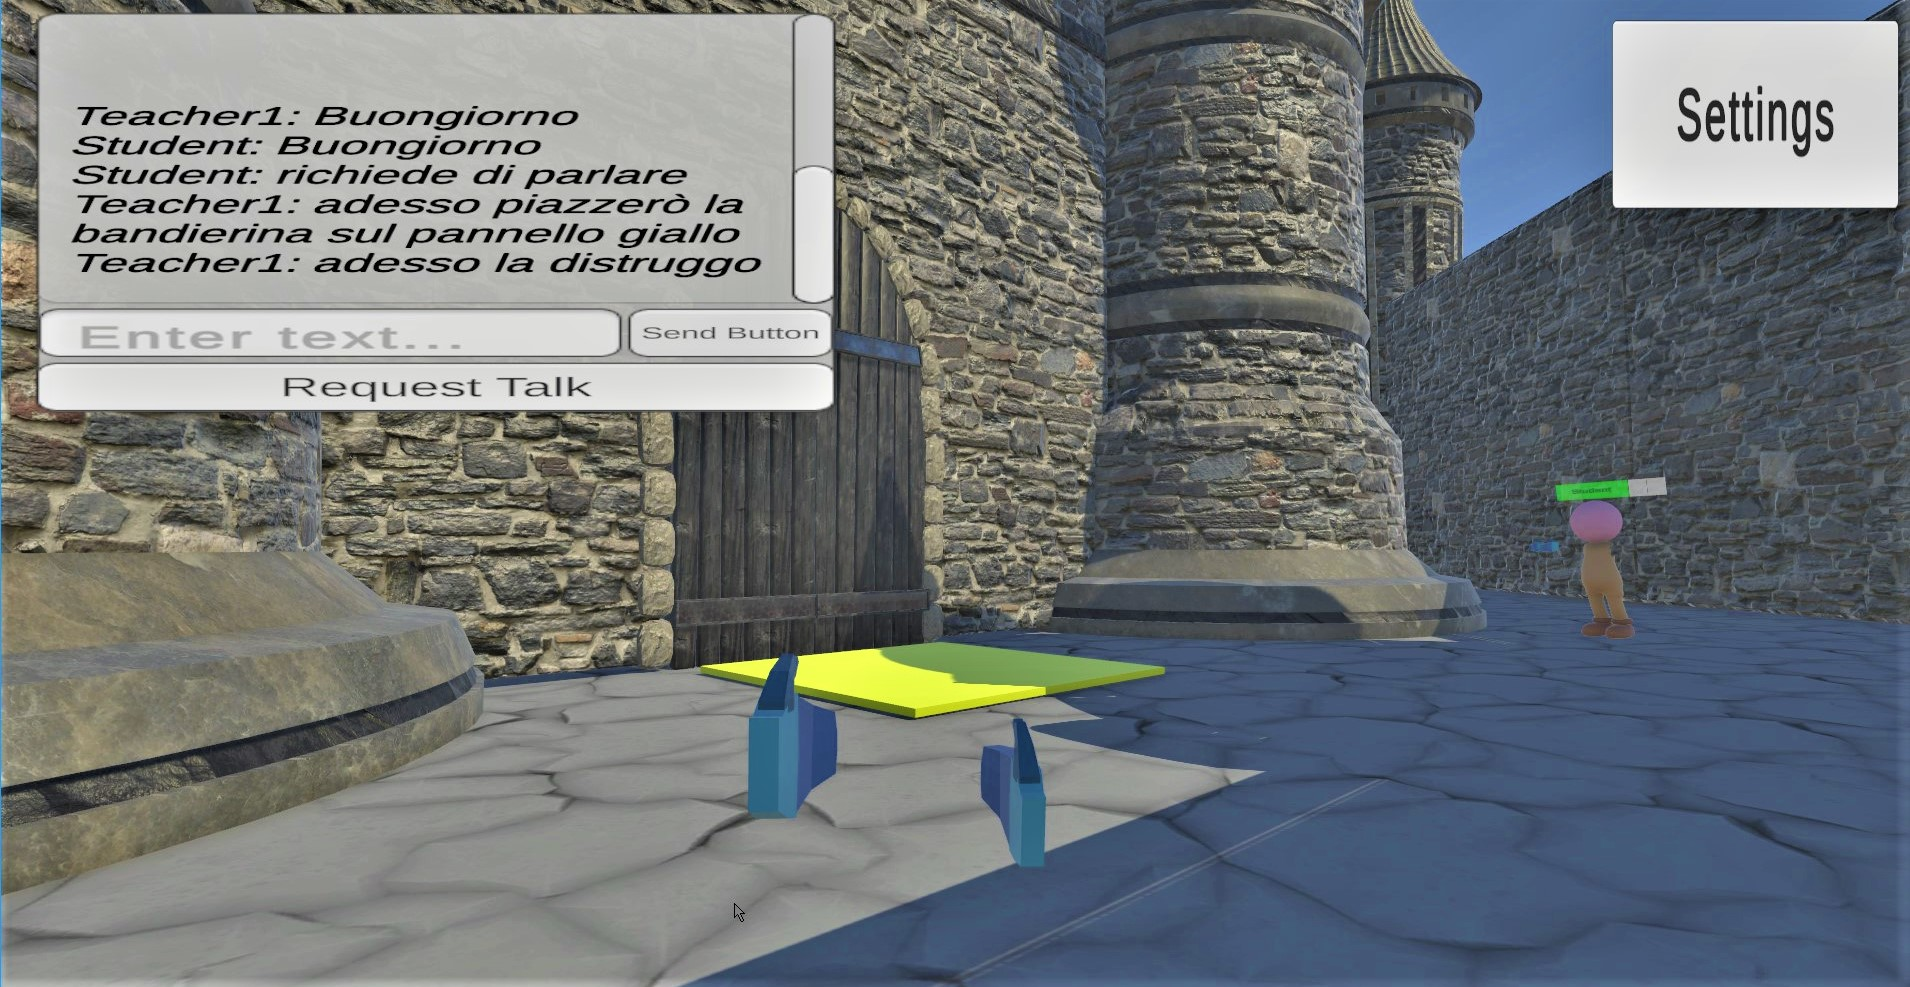
\includegraphics[scale = 0.25]{Immagini/Dimostrazioni d'uso/bandierinadistruttalatodoc.jpg}
\caption{Scena dopo la distruzione della bandierina lato docente}
\end{figure}
\begin{figure}[H]
\centering
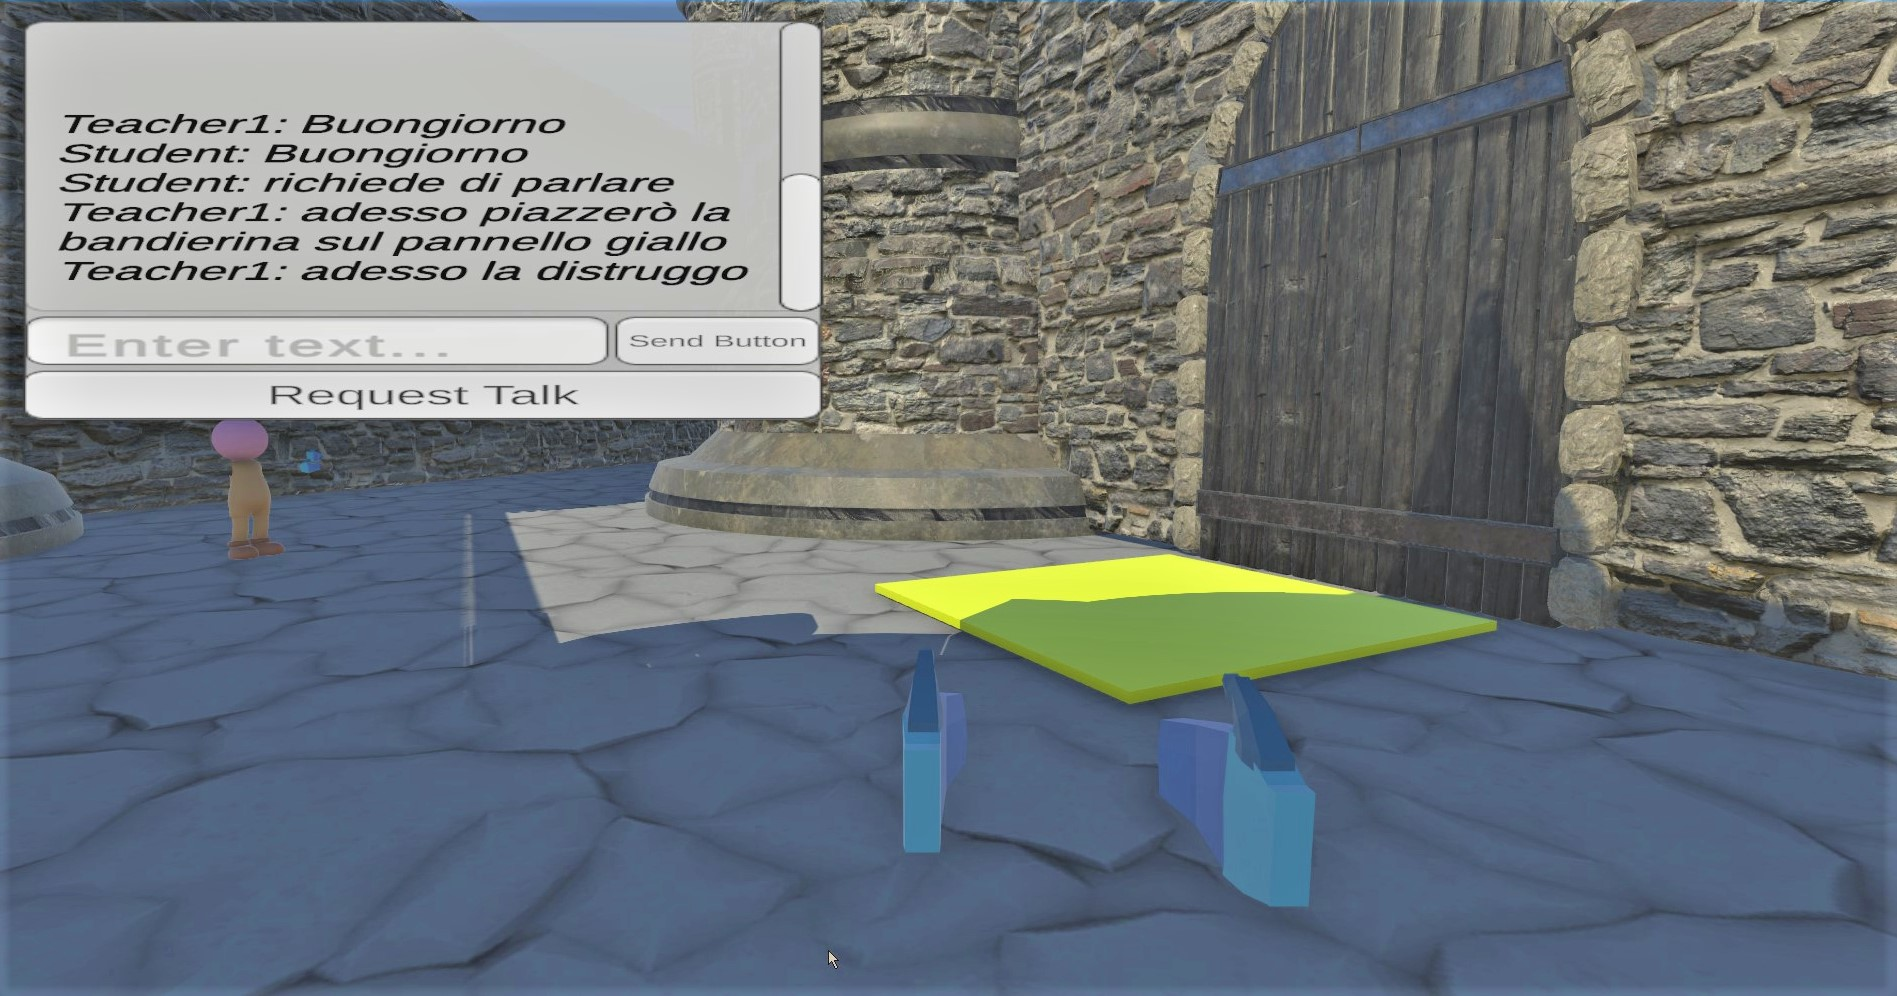
\includegraphics[scale = 0.25]{Immagini/Dimostrazioni d'uso/bandierinadistruttalatostud.jpg}
\caption{Scena dopo la distruzione della bandierina lato studente}
\end{figure}
\chapter{Sviluppi futuri}
Nei capitoli precedenti sono state illustrate le fasi del progetto, partendo dai requisiti che sono stati fissati fino allo sviluppo delle funzionalità vere e proprie del \textit{software}.
Il progetto descritto in questa relazione è, appunto, un prototipo, quindi ha molti aspetti che, in futuro, potranno essere migliorati e altri elementi che potranno essere aggiunti al fine di renderlo un prodotto effettivamente utilizzabile a scopi didattici.
\section{Sviluppi Futuri}
Saranno ora illustrati alcuni aspetti che sono stati pensati per arricchire e migliorare il prototipo.
\\Le funzionalità che verranno descritte rappresentano una piccola parte rispetto a tutte quelle che si possono ideare, come è ben noto il mondo della progettazione e sviluppo \textit{software} è ricco di possibilità e alternative.
\subsection{Visibilità dei Raggi}
Si prenda, per esempio, uno studente che voglia chiedere informazioni su un punto preciso della scena, tramite la chat vocale o scritta potrebbe risultare complesso dare indicazioni precise sul punto che vuole mettere in risalto, visto che con quegli strumenti non può mostrare agli utenti quello che lui sta visualizzando nel proprio visore. 
\\Per facilitare questa operazione, potrà essere estremamente utile rendere i raggi di ogni giocatore visibili anche agli altri utenti nella scena. 
\\In questo modo, se uno studente volesse indicare con uno dei due raggi un punto preciso, anche gli atri utenti vedranno il raggio dello studente che sta indicando quel punto.
\subsection{Avatar realistici}
In questo momento, per rappresentare gli utenti in scena, è presente un \textit{\gls{avatar}} stilizzato di un essere umano.
\\In futuro si potrebbero implementare i seguenti miglioramenti:
\begin{itemize}
    \item Un \textit{avatar} che sia simile, il più possibile, ad un essere umano;
    \item Movimenti delle braccia e delle gambe dell'\textit{avatar} quando l'utente muove i \textit{controller} o si muove nella scena;
    \item Più modelli di \textit{avatar}, in modo che un utente possa scegliere quello che più desidera.
\end{itemize}
\subsection{Ambientazione esistente}
Lo scenario finale, in cui tutti i giocatori si muovono e interagiscono, rappresenta un castello medioevale, con due piccoli villaggi ai lati, immerso nella natura.
\\Nell'introduzione è stato spiegato questo scenario è fittizio, siccome lo scopo del progetto è quello di immergere gli utenti in uno scenario reale, in futuro sarà sicuramente necessario importare la rappresentazione digitale di un'ambientazione esistente.
\subsection{Sistema di Registrazione e Autenticazione}
Un'altra meccanica sicuramente migliorabile è quella della registrazione e dell'autenticazione dell'utente.
\\Per quanto riguarda l'insegnate, è presente un file con alcune coppie utente/password per poter passare dalla scena iniziale alla lobby insegnante.
\\Per lo studente, invece, non è presente alcun tipo di autenticazione vera e propria, deve solo inserire una qualsiasi stringa nel campo apposito per poter passare dalla scena iniziale alla lobby studente.
\\Inoltre, non è presente un sistema per la registrazione in un database dello \textit{username} degli utenti, questo problema comporta la possibile presenza di due o più utenti con lo stesso \textit{username}.
\\Esistono alcune aziende che offrono una soluzione per l'aggiunta un sistema di registrazione e autenticazione degli utenti per le applicazioni, una di queste è \textbf{Auth0} \footnote{(\url{https://auth0.com/}) sito web di Auth0}.
\printbibliography[heading=bibintoc, title={Bibliografia e Sitografia}]
\end{document}